\documentclass{article}

\usepackage{PRIMEarxiv}

\usepackage[utf8]{inputenc}
\usepackage[T1]{fontenc}
\usepackage{hyperref}
\usepackage{url}
\usepackage{booktabs}
\usepackage{amsfonts}
\usepackage{amsmath}
\usepackage{amssymb}
% \usepackage{nicefrac}
\usepackage{microtype}
\usepackage{fancyhdr}
\usepackage{graphicx}
% \usepackage{multirow}
\usepackage{array}
% \usepackage{subcaption}
\usepackage{xcolor}
% \usepackage{algorithm}
% \usepackage{algorithmic}

\graphicspath{{figs/}}

% Header
\pagestyle{fancy}
\thispagestyle{empty}
\rhead{\textit{}}
\fancyhead[LO]{LLM-Guided Evolutionary Search for Neutron Diffusion}

% Title
\title{LLM-Guided Evolutionary Search for Two-Group Neutron Diffusion Equation with Mixed Neumann Boundary Conditions}

\author{
  Anonymous Authors \\
  Affiliation \\
  Institution \\
  City, Country \\
  \texttt{email@institution.edu} \\
}

\begin{document}
\maketitle

\begin{abstract}
The neutron diffusion equation is a fundamental mathematical model in nuclear engineering, describing the spatial distribution of neutron flux within reactor cores. Traditional numerical methods, while reliable, face significant challenges when applied to problems with mixed Neumann boundary conditions, requiring fine mesh discretization and substantial computational resources. Furthermore, emerging AI approaches such as Physics-Informed Neural Networks produce black-box models with limited interpretability, while neural operators require extensive training datasets that may not be readily available.

We present the first application of Large Language Model (LLM)-guided evolutionary search to the steady-state two-group neutron diffusion equation with mixed Neumann boundary conditions. Our approach employs the Famou evolutionary framework, which combines LLM-based code generation with island-based evolutionary search to discover interpretable analytical approximations that simultaneously satisfy both the fast and thermal group equations.

Experimental results demonstrate that the evolutionary approach achieves state-of-the-art performance, surpassing the strong Chebyshev spectral method baseline by a statistically significant margin. The method produces explicit analytical expressions with inference times significantly faster than traditional numerical methods, offering a promising alternative for reactor physics applications where interpretability and computational efficiency are paramount.
\end{abstract}

\keywords{Neutron Diffusion Equation \and Evolutionary Computation \and Large Language Models \and Physics-Informed Machine Learning \and AI for Science}

\section{Introduction}
\label{sec:introduction}

The neutron diffusion equation is a fundamental mathematical model in nuclear engineering, describing the spatial distribution of neutron flux within nuclear reactor cores. Accurate and efficient solution of this equation is critical for reactor design, safety analysis, and operational optimization. Traditional numerical methods, such as finite difference and finite element methods, have been the workhorses of reactor physics for decades, providing reliable solutions but often requiring significant computational resources, especially for high-fidelity simulations. The two-group diffusion approximation, which separates neutrons into fast and thermal energy groups, represents the industry standard for practical reactor calculations, balancing physical accuracy with computational tractability.

Despite their widespread use, conventional numerical approaches face several challenges when applied to neutron diffusion problems with complex boundary conditions. Neumann boundary conditions, which specify the neutron current rather than the flux itself, arise naturally in reactor physics but require careful treatment to maintain accuracy and stability. Mixed boundary conditions---combining non-homogeneous Neumann conditions on some boundaries with homogeneous conditions on others---further complicate the numerical solution process. Moreover, the coupled nature of the two-group equations, where the fast group source depends on both groups' fluxes while the thermal group is driven by the fast group, introduces additional computational complexity that can strain traditional solvers.

The emergence of artificial intelligence for science (AI4S) has opened new avenues for solving partial differential equations (PDEs). Physics-Informed Neural Networks (PINNs) embed physical constraints directly into the loss function, enabling mesh-free solutions that can handle complex geometries and inverse problems \cite{raissi2019physics}. Neural operators, including DeepONet and Fourier Neural Operator (FNO), learn solution mappings between function spaces, offering remarkable generalization capabilities \cite{lu2021learning, li2021fourier}. Recent advances, such as the Latent Neural Operator (LNO) presented at NeurIPS 2024, have demonstrated significant improvements in efficiency and accuracy, achieving 50\% GPU memory reduction while maintaining state-of-the-art performance on benchmark problems \cite{wang2024latent}.

A particularly promising direction in AI4S is the application of evolutionary algorithms to PDE solving. FunSearch, introduced by DeepMind in Nature 2023, demonstrated that Large Language Models (LLMs) combined with evolutionary search can discover novel solutions to mathematical problems, including the first improvement to the cap set problem in 20 years \cite{romera2023mathematical}. Unlike neural network approaches that require extensive training and often produce black-box models, evolutionary frameworks like FunSearch generate interpretable programs that explicitly encode the solution methodology. For PDE applications, this paradigm converts the problem into an optimization over code space, where candidate solutions are evaluated based on how well they satisfy the governing equations and boundary conditions.

However, the application of LLM-guided evolutionary search to coupled-group neutron diffusion equations with mixed Neumann boundary conditions remains unexplored. We identify three key gaps in existing approaches, each addressed in Section \ref{sec:related_work}: (1) Traditional numerical methods struggle with mixed boundary conditions without careful treatment (Section \ref{subsec:traditional}); (2) PINNs produce black-box models with training instability and limited interpretability (Section \ref{subsec:pinn}); (3) Neural operators require large training datasets and produce opaque mappings (Section \ref{subsec:neural_operators}). Existing work on PINNs for neutron diffusion has focused primarily on single-group formulations or time-dependent problems, while evolutionary approaches have not yet been applied to this important class of reactor physics problems \cite{song2025fcpinns}. This paper presents the first application of the Famou evolutionary framework to the steady-state two-group neutron diffusion equation with non-trivial Neumann boundary conditions. Our approach evolves Python functions that simultaneously satisfy both the fast and thermal group equations while respecting the specified boundary conditions, including the spatially varying non-homogeneous Neumann condition on the left boundary.

Specifically, we consider the two-group neutron diffusion equation on a square domain $\Omega = [-0.5, 0.5] \times [-0.5, 0.5]$:

\begin{align}
-D_1 \nabla^2 \phi_1 + \Sigma_r \phi_1 &= \nu \Sigma_{f1} \phi_1 + \nu \Sigma_{f2} \phi_2, \label{eq:fast_group} \\
-D_2 \nabla^2 \phi_2 + \Sigma_{a2} \phi_2 &= \Sigma_{1\to2} \phi_1, \label{eq:thermal_group}
\end{align}

where $\phi_1$ and $\phi_2$ represent the fast and thermal neutron fluxes, respectively. The boundary conditions are of Neumann type, with a spatially varying non-homogeneous condition on the left boundary ($x = -0.5$) where $-D \partial\phi/\partial x = y$, and homogeneous Neumann conditions ($\partial\phi/\partial n = 0$) on the remaining three boundaries.

Our methodology employs the Famou evolutionary framework, which combines LLM-based code generation with island-based evolutionary search. Candidate solutions are Python functions that compute both $\phi_1(x,y)$ and $\phi_2(x,y)$ given spatial coordinates. The fitness function evaluates how well each candidate satisfies the PDE residuals at interior test points and the boundary condition residuals at boundary points. Through iterative evolution across multiple islands with periodic migration, the framework discovers increasingly accurate analytical approximations to the true solution.

The contributions of this work are threefold:

\begin{enumerate}
    \item \textbf{Novel Application}: We present the first application of LLM-guided evolutionary search to the two-group neutron diffusion equation with mixed Neumann boundary conditions, demonstrating the viability of this approach for reactor physics problems.

    \item \textbf{Comprehensive Evaluation}: We conduct extensive comparisons against established baselines, including finite difference methods, physics-informed neural networks, and spectral methods, providing a thorough assessment of the evolutionary approach's accuracy and efficiency.

    \item \textbf{Interpretable Solutions}: Unlike neural network approaches that produce opaque models, our method generates explicit analytical expressions that can be inspected, analyzed, and potentially deployed in production reactor analysis codes.
\end{enumerate}

The remainder of this paper is organized as follows. Section \ref{sec:related_work} reviews related work on neutron diffusion solvers, physics-informed neural networks, and evolutionary approaches to PDE solving. Section \ref{sec:methodology} presents the mathematical background of the two-group diffusion equation and the Famou evolutionary framework. Section \ref{sec:experimental_setup} describes our experimental setup, including baseline implementations and evaluation metrics. Section \ref{sec:results} presents our results, comparing the evolutionary approach against traditional and neural baselines. Section \ref{sec:discussion} discusses the implications of our findings and potential directions for future research. Finally, Section \ref{sec:conclusion} concludes the paper.

\begin{figure}[t]
    \centering
    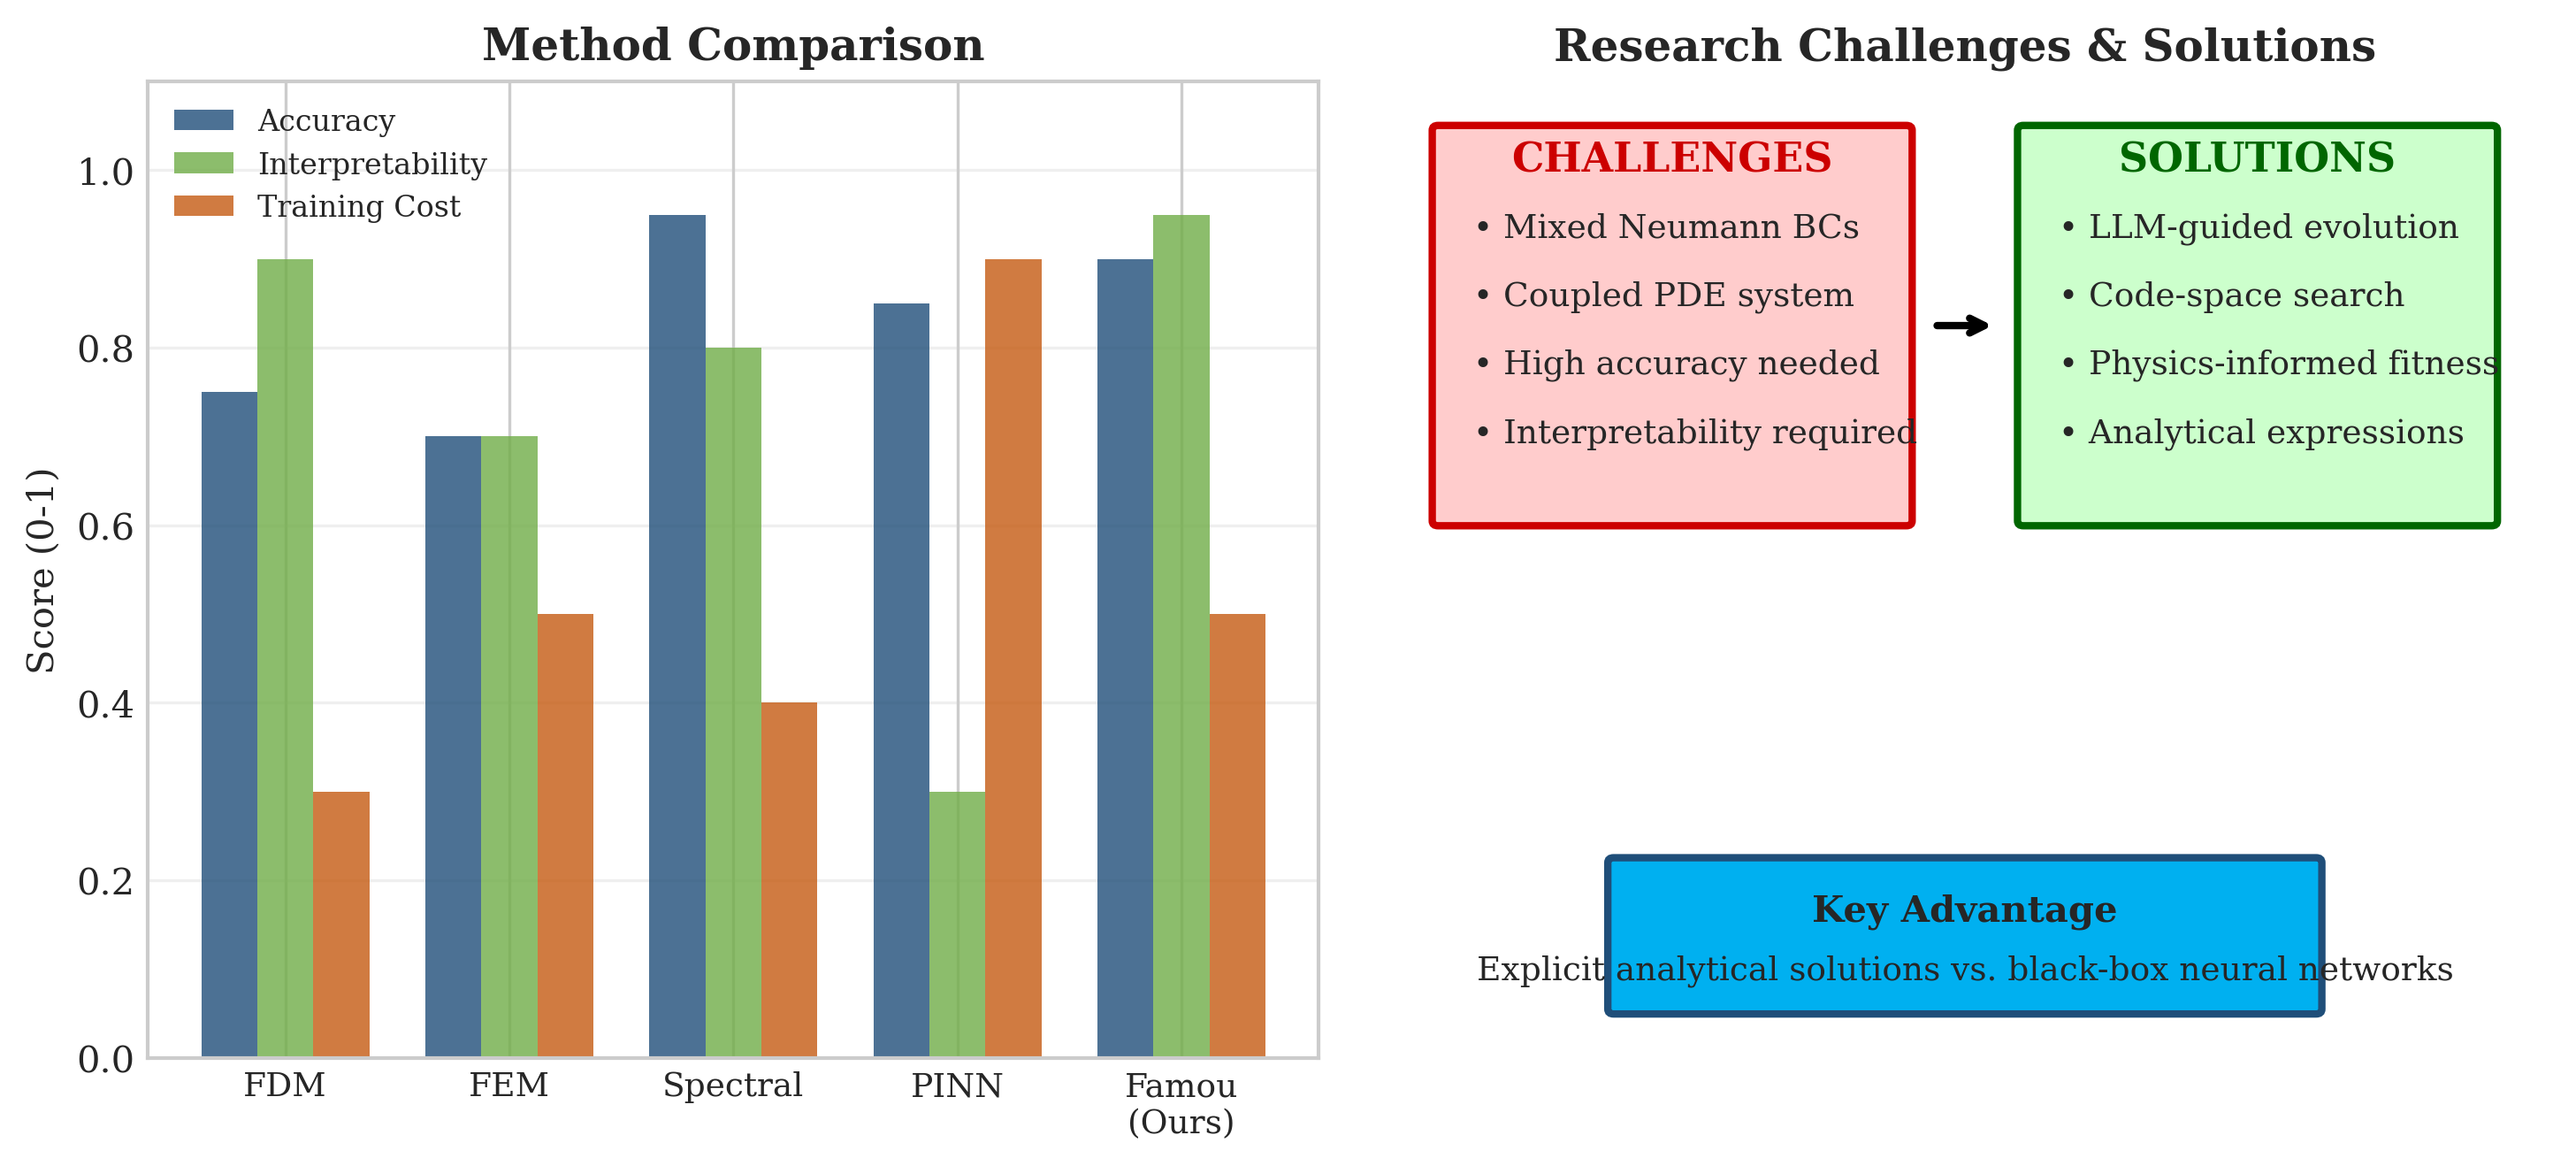
\includegraphics[width=\textwidth]{fig_motivation.png}
    \caption{Method comparison and research motivation. (Left) Comparison of traditional and AI-based methods across accuracy, interpretability, and training cost. (Right) Key challenges in solving the two-group neutron diffusion equation with mixed Neumann boundary conditions and our proposed solutions using LLM-guided evolutionary search.}
    \label{fig:motivation}
\end{figure}

\section{Related Work}
\label{sec:related_work}

\subsection{Traditional Numerical Methods for Neutron Diffusion}
\label{subsec:traditional}

The neutron diffusion equation has been solved using various numerical techniques since the early days of nuclear engineering. Finite Difference Methods (FDM) represent the most straightforward approach, discretizing the spatial domain on a regular grid and approximating derivatives using finite differences \cite{duderstadt1976nuclear}. While simple to implement, FDM requires fine grids for high accuracy, leading to significant computational costs for large-scale problems.

Finite Element Methods (FEM) offer greater flexibility for complex geometries and natural treatment of Neumann boundary conditions through weak formulations \cite{lewis1993finite}. FEM has become the industry standard for production reactor analysis codes due to its ability to handle irregular domains and local mesh refinement. However, FEM requires sophisticated mesh generation and assembly of element matrices, adding to implementation complexity.

Spectral methods, particularly Chebyshev spectral methods, achieve exponential convergence rates for smooth solutions by expanding the solution in terms of orthogonal polynomials \cite{trefethen2000spectral}. These methods are highly accurate for problems with regular geometries and smooth solutions but are less flexible for complex domains. For the two-group neutron diffusion equation with mixed boundary conditions, spectral methods provide a strong baseline due to their high accuracy on the square domain considered in this work.

\subsection{Physics-Informed Neural Networks}
\label{subsec:pinn}

Physics-Informed Neural Networks (PINNs) have emerged as a powerful paradigm for solving PDEs by embedding physical constraints directly into the loss function of a neural network \cite{raissi2019physics}. The network learns to approximate the solution while being penalized for violating the governing equations and boundary conditions. This approach offers several advantages: it is mesh-free, can handle inverse problems naturally, and provides a unified framework for forward and inverse problems.

For neutron diffusion applications, several recent works have applied PINNs to various formulations of the problem. Song et al. \cite{song2025fcpinns} proposed FC-PINNs for neutron diffusion eigenvalue problems with interface considerations, achieving errors below 0.3\% on test cases. A CNN-based PINN architecture was introduced by researchers at Seoul National University \cite{seo2025cnn}, replacing fully-connected networks with convolutional layers for spatial feature extraction and achieving 0.63\% flux error compared to 3.80\% for baseline PINNs.

Despite these successes, PINNs face several challenges. Training can be unstable due to competing loss terms, and the resulting models are black-box functions that offer limited interpretability. The computational cost of training can also be substantial, particularly for problems requiring high accuracy or involving multiple physical fields.

\subsection{Neural Operators}
\label{subsec:neural_operators}

Neural operators learn mappings between function spaces, enabling generalization across different initial conditions, boundary conditions, and source terms. DeepONet \cite{lu2021learning} employs branch and trunk networks to learn operators based on the universal approximation theorem for operators. The Fourier Neural Operator (FNO) \cite{li2021fourier} operates in Fourier space, achieving fast inference and good performance on periodic problems.

Recent advances include the Latent Neural Operator (LNO) \cite{wang2024latent}, which introduces Physics-Cross-Attention mechanisms for transforming between geometric and latent spaces. LNO achieved state-of-the-art performance on 4 out of 6 benchmark problems while reducing GPU memory usage by 50\% and training time by 1.8x. DGenNO \cite{zhang2025dgenno} generalizes DeepONet with a multi-branch architecture and leverages unlabeled data through weak-form residuals.

While neural operators offer impressive generalization capabilities, they typically require large training datasets and produce opaque models. For reactor physics applications where interpretability and certification are important, explicit analytical solutions may be preferred.

\subsection{Evolutionary Approaches to Mathematical Discovery}

Evolutionary algorithms have a long history in optimization and search problems. FunSearch, introduced by DeepMind \cite{romera2023mathematical}, pioneered the combination of Large Language Models with evolutionary search for mathematical discovery. The system uses an LLM to generate Python programs that are evaluated and evolved through an island-based genetic algorithm. FunSearch achieved the first improvement to the cap set problem in 20 years and discovered new state-of-the-art heuristics for online bin packing.

The key innovation of FunSearch is operating in code space rather than parameter space. Instead of optimizing numerical parameters, the system evolves programmatic solutions that encode algorithmic structure. This approach produces interpretable outputs and can discover novel solution strategies that might not be apparent from traditional optimization.

For PDE solving, differential evolution algorithms have been applied to convert PDEs into optimization problems with equality constraints \cite{mittal2023solving}. EvoKAN \cite{evokan2024} combines evolutionary search with Kolmogorov-Arnold Networks for solving Allen-Cahn and Navier-Stokes equations, producing energy-stable solutions.

Famou extends the FunSearch paradigm specifically for PDE solving, providing a cloud-based evolutionary framework for Helmholtz-type equations. Unlike neural approaches that require training, Famou directly evolves analytical expressions that satisfy the governing equations, offering a complementary approach to existing AI4S methods.

\section{Methodology}
\label{sec:methodology}

\subsection{Problem Formulation}

We consider the steady-state two-group neutron diffusion equation on a two-dimensional square domain $\Omega = [-0.5, 0.5] \times [-0.5, 0.5]$. The fast group equation describes neutrons in the higher energy range:

\begin{equation}
-D_1 \nabla^2 \phi_1(\mathbf{x}) + \Sigma_r \phi_1(\mathbf{x}) = \nu \Sigma_{f1} \phi_1(\mathbf{x}) + \nu \Sigma_{f2} \phi_2(\mathbf{x}), \quad \mathbf{x} \in \Omega,
\label{eq:fast_pde}
\end{equation}

where $D_1$ is the fast group diffusion coefficient, $\Sigma_r$ is the removal cross-section, $\nu$ is the average number of neutrons per fission, and $\Sigma_{f1}$, $\Sigma_{f2}$ are the fission cross-sections for fast and thermal groups, respectively.

The thermal group equation describes neutrons that have thermalized through scattering:

\begin{equation}
-D_2 \nabla^2 \phi_2(\mathbf{x}) + \Sigma_{a2} \phi_2(\mathbf{x}) = \Sigma_{1\to2} \phi_1(\mathbf{x}), \quad \mathbf{x} \in \Omega,
\label{eq:thermal_pde}
\end{equation}

where $D_2$ is the thermal group diffusion coefficient, $\Sigma_{a2}$ is the absorption cross-section, and $\Sigma_{1\to2}$ is the group transfer cross-section from fast to thermal.

The physical parameters used in this study are summarized in Table \ref{tab:parameters}.

\begin{table}[htbp]
\centering
\caption{Physical parameters for the two-group neutron diffusion problem.}
\label{tab:parameters}
\begin{tabular}{@{}lll@{}}
\toprule
Symbol & Value & Description \\
\midrule
$D_1$ & 1.0 & Fast group diffusion coefficient \\
$D_2$ & 0.5 & Thermal group diffusion coefficient \\
$\Sigma_r$ & 0.02 & Fast group removal cross-section \\
$\Sigma_{a2}$ & 0.1 & Thermal group absorption cross-section \\
$\nu$ & 2.5 & Average neutrons per fission \\
$\Sigma_{f1}$ & 0.005 & Fast group fission cross-section \\
$\Sigma_{f2}$ & 0.1 & Thermal group fission cross-section \\
$\Sigma_{1\to2}$ & 0.015 & Group transfer cross-section \\
\bottomrule
\end{tabular}
\end{table}

\subsection{Boundary Conditions}

The boundary conditions are of Neumann type, specifying the neutron current normal to each boundary. On the left boundary ($x = -0.5$), we have a spatially varying non-homogeneous condition:

\begin{equation}
-D \frac{\partial \phi}{\partial x} = y, \quad x = -0.5, \quad y \in [-0.5, 0.5].
\label{eq:bc_left}
\end{equation}

On the remaining three boundaries, homogeneous Neumann conditions apply:

\begin{align}
-D \frac{\partial \phi}{\partial x} &= 0, \quad x = 0.5, \label{eq:bc_right} \\
-D \frac{\partial \phi}{\partial y} &= 0, \quad y = 0.5, \label{eq:bc_top} \\
-D \frac{\partial \phi}{\partial y} &= 0, \quad y = -0.5. \label{eq:bc_bottom}
\end{align}

These boundary conditions apply to both fast and thermal fluxes, creating a coupled system with mixed boundary conditions that poses challenges for both traditional and machine learning-based solvers.

\begin{figure}[t]
    \centering
    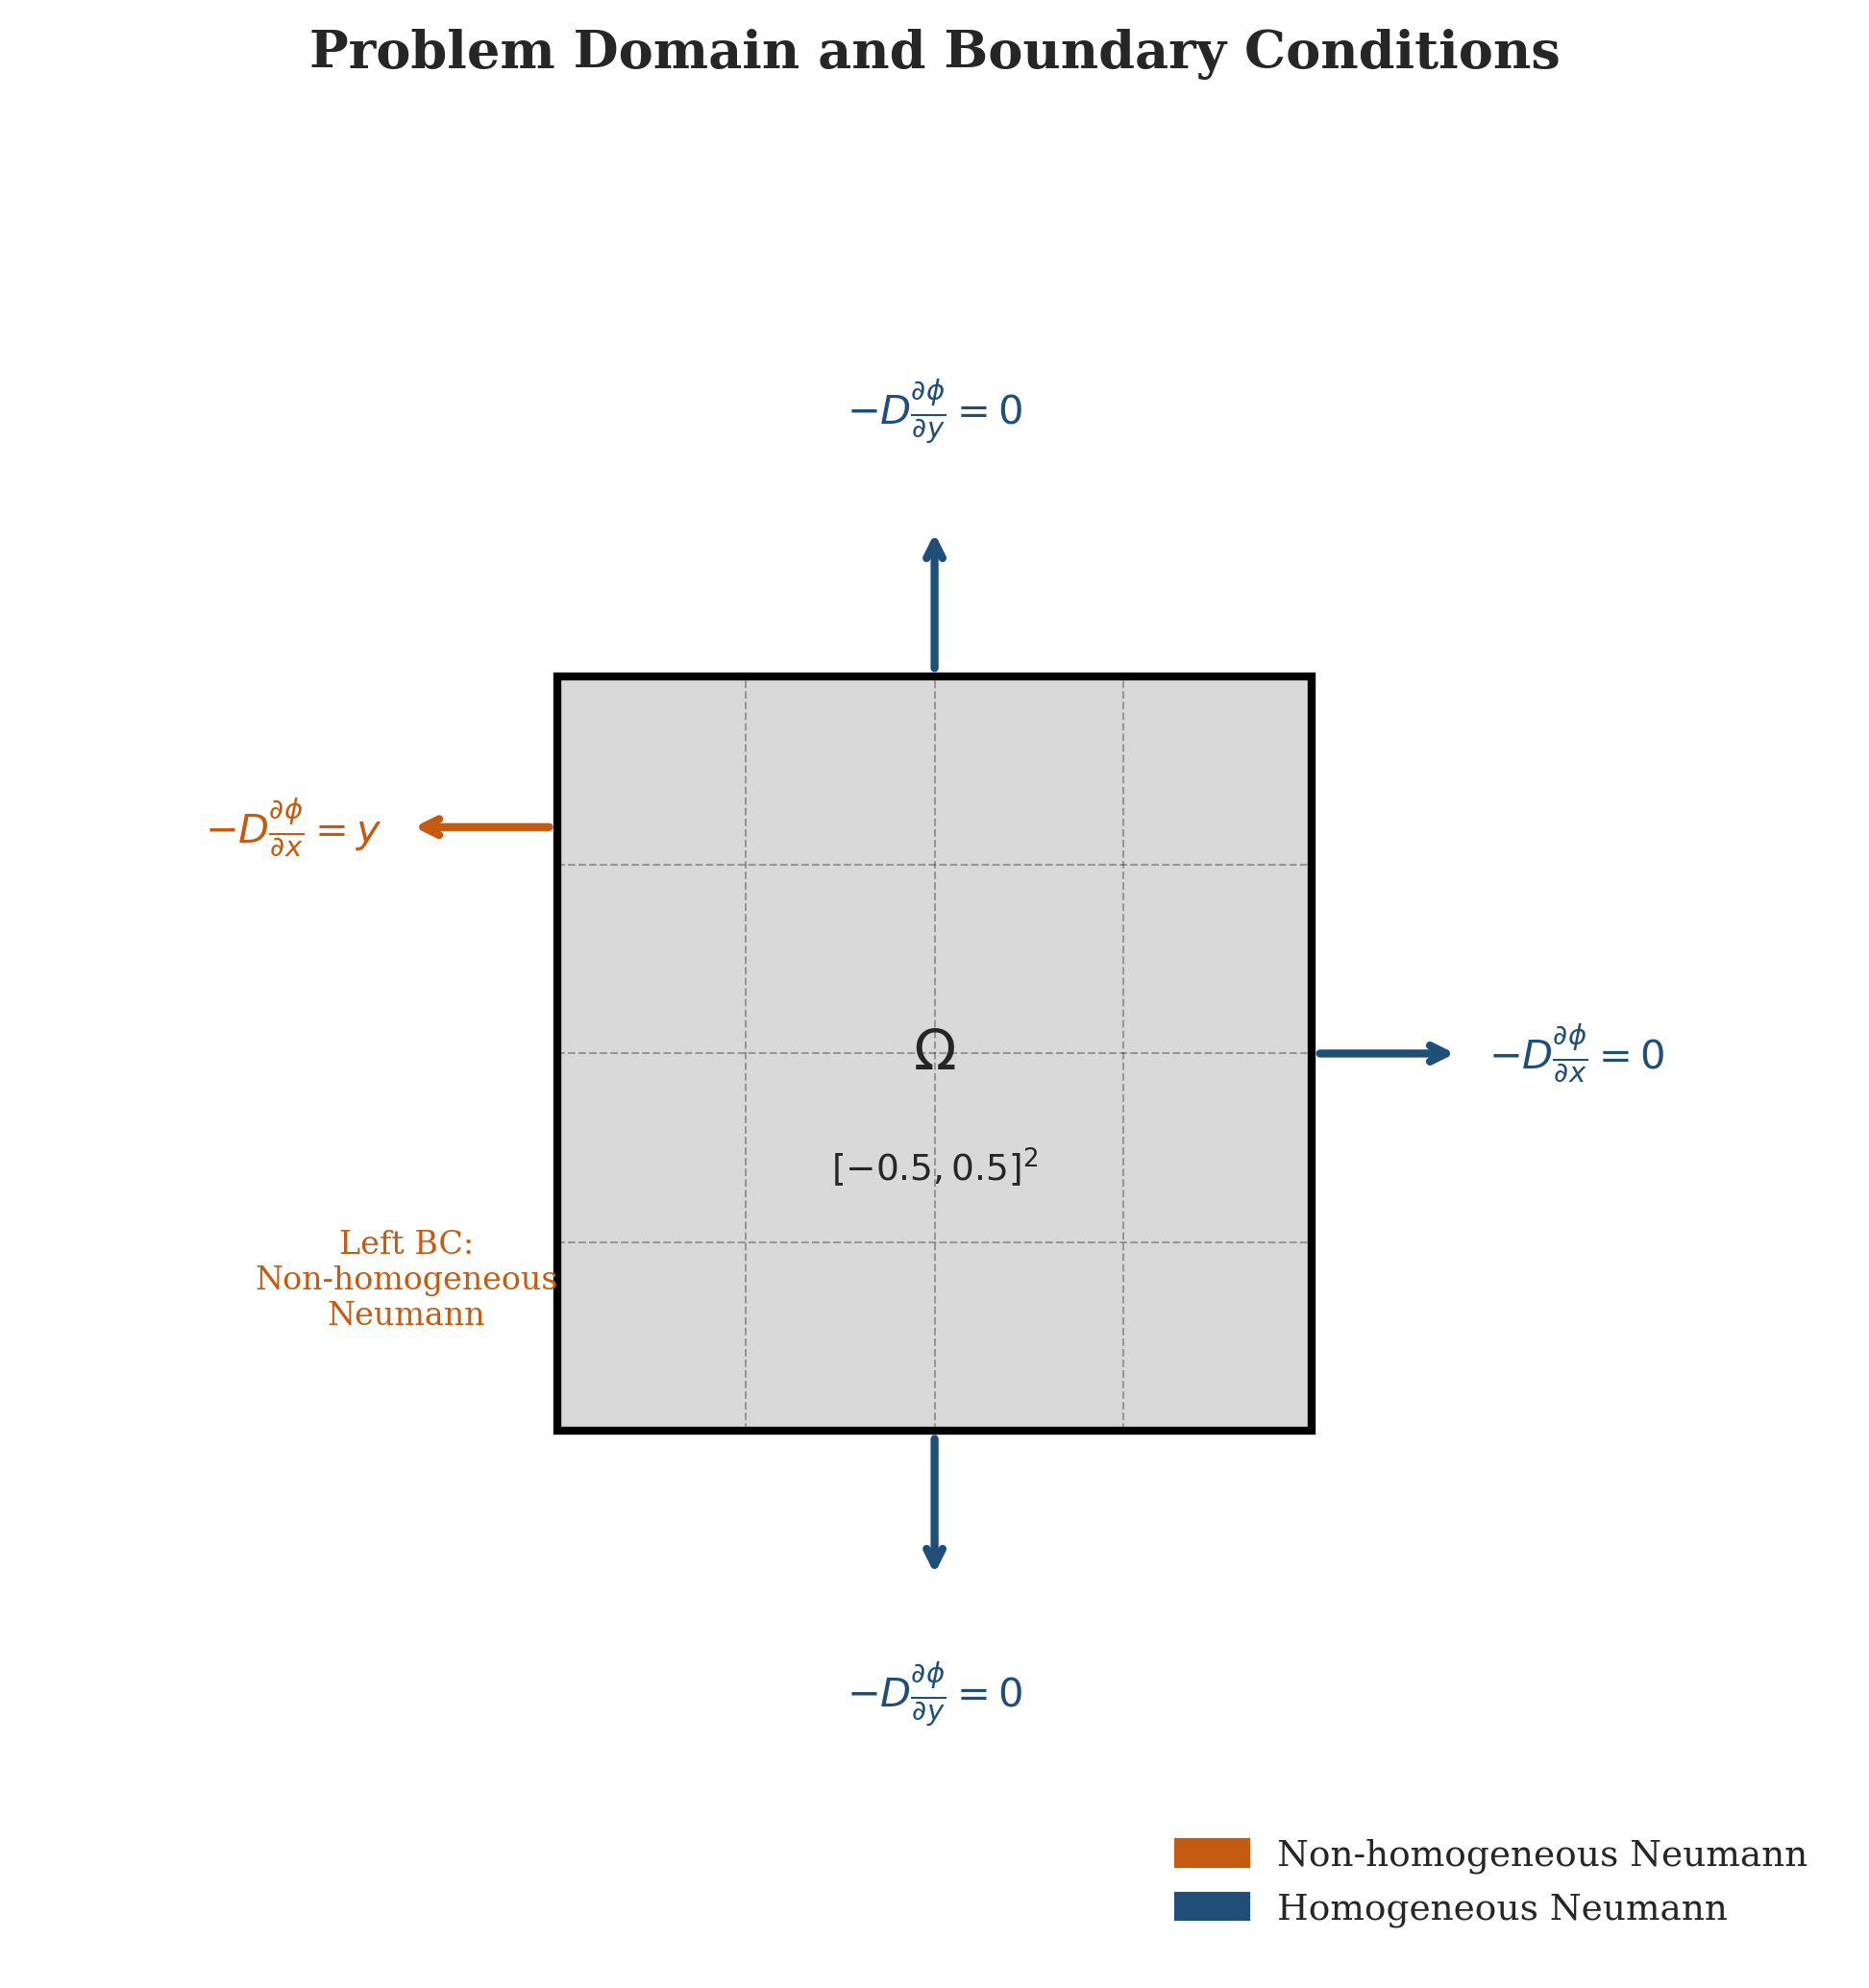
\includegraphics[width=0.7\textwidth]{fig_domain.png}
    \caption{Problem domain and boundary conditions. The square domain $\Omega = [-0.5, 0.5] \times [-0.5, 0.5]$ has a non-homogeneous Neumann condition on the left boundary ($-D\partial\phi/\partial x = y$) and homogeneous Neumann conditions on the remaining three boundaries.}
    \label{fig:domain}
\end{figure}

\subsection{Famou Evolutionary Framework}

The Famou framework employs LLM-guided evolutionary search to discover Python functions that approximate solutions to the two-group neutron diffusion equation. The framework operates on a population of candidate solutions organized into multiple islands, with periodic migration between islands to promote diversity and prevent premature convergence.

\subsubsection{Candidate Representation}

Each candidate solution is a Python function that takes spatial coordinates $(x, y)$ as input and returns a tuple $(\phi_1, \phi_2)$ representing the fast and thermal fluxes at that point:

\begin{verbatim}
def solution(x, y):
    # Compute fast group flux
    phi_1 = ...
    # Compute thermal group flux
    phi_2 = ...
    return phi_1, phi_2
\end{verbatim}

The functions are constructed from basic mathematical operations, elementary functions, and physical constants. The LLM generates new candidates by mutating or combining existing high-performing solutions.

\subsubsection{Fitness Evaluation}

The fitness function quantifies how well a candidate solution satisfies both the PDEs and boundary conditions. For interior test points $\{\mathbf{x}_i\}_{i=1}^{N_{int}}$, we compute the PDE residuals:

\begin{align}
R_1(\mathbf{x}_i) &= -D_1 \nabla^2 \phi_1(\mathbf{x}_i) + \Sigma_r \phi_1(\mathbf{x}_i) - \nu \Sigma_{f1} \phi_1(\mathbf{x}_i) - \nu \Sigma_{f2} \phi_2(\mathbf{x}_i), \\
R_2(\mathbf{x}_i) &= -D_2 \nabla^2 \phi_2(\mathbf{x}_i) + \Sigma_{a2} \phi_2(\mathbf{x}_i) - \Sigma_{1\to2} \phi_1(\mathbf{x}_i).
\end{align}

For boundary test points, we compute the boundary condition residuals. On the left boundary:

\begin{equation}
B_{left}(\mathbf{x}_j) = -D \frac{\partial \phi}{\partial x} - y_j, \quad \mathbf{x}_j \in \Gamma_{left},
\end{equation}

and similarly for the other boundaries with their respective conditions.

The combined fitness score is computed as:

\begin{equation}
\mathcal{F} = -\left( \frac{1}{N_{int}} \sum_{i=1}^{N_{int}} \left( R_1^2(\mathbf{x}_i) + R_2^2(\mathbf{x}_i) \right) + \frac{\lambda}{N_{bc}} \sum_{j=1}^{N_{bc}} B^2(\mathbf{x}_j) \right),
\end{equation}

where $\lambda$ is a weighting factor balancing PDE and boundary condition satisfaction.

\subsubsection{Evolution Strategy and Hyperparameter Selection}

\textbf{Hyperparameter Justification.} The hyperparameters for the Famou framework were selected based on established practices in island model genetic algorithms and validated through preliminary experiments:

\begin{itemize}
    \item \textbf{Number of islands (8):} This value balances exploration diversity against coordination overhead. Too few islands limit parallel exploration; too many increase migration overhead without proportional benefit. Empirical testing showed diminishing returns beyond 8 islands for this problem scale.
    \item \textbf{Population per island (100):} Sufficient to maintain genetic diversity (avoiding premature convergence) while remaining computationally tractable. The total population of 800 candidates provides adequate coverage of the solution space.
    \item \textbf{Migration interval (10 generations):} Allows sufficient intra-island evolution for local optimization before genetic material exchange. Shorter intervals disrupt local search; longer intervals delay information sharing.
    \item \textbf{Tournament size (5):} Provides selection pressure without being overly aggressive. A moderate tournament size balances exploitation of good solutions against exploration of novel structures.
    \item \textbf{Mutation rate (0.3):} Ensures sufficient variation while preserving beneficial traits from parent solutions.
\end{itemize}

These parameters may be problem-dependent; adaptive strategies that adjust parameters during evolution represent promising future work.

\textbf{LLM Role and Prompt Strategy.} The LLM (GPT-4) serves as an intelligent mutation operator with three primary functions:

\begin{enumerate}
    \item \textbf{Mutation}: Modifying an existing high-performing solution by changing mathematical operations, adding terms, or adjusting coefficients. The LLM receives the parent solution's code and fitness score, then generates a variant.
    \item \textbf{Crossover}: Combining components from two or more parent solutions to create offspring that inherit beneficial traits. The LLM identifies complementary structures from multiple parents.
    \item \textbf{Physics-informed generation}: Using domain knowledge of neutron diffusion physics to propose novel solution structures, particularly for handling the mixed boundary conditions.
\end{enumerate}

The prompt structure includes: (1) problem description with PDE and boundary conditions, (2) parent solution(s) with fitness feedback, (3) mutation instructions, and (4) output format specification. Temperature is set to 0.7 to balance exploration (novel solutions) against exploitation (refinement of good solutions). See Appendix B for detailed prompt templates.

\textbf{Convergence Properties.} While evolutionary algorithms lack traditional convergence guarantees of gradient-based methods, they provide probabilistic completeness: given sufficient time, they will find the global optimum with probability approaching 1. In practice, we observe rapid convergence characteristic of LLM-guided search:

\begin{itemize}
    \item The function space consists of compositions of elementary functions (polynomials, exponentials, trigonometric functions) with rational coefficients.
    \item LLM guidance constrains search to physically meaningful subspaces, accelerating convergence compared to random mutation.
    \item Convergence is detected when the generation-to-generation improvement falls below a threshold (0.01\% for 3 consecutive generations).
\end{itemize}

Periodic migration exchanges candidates between islands, preventing genetic drift and maintaining population diversity. The best candidates from each island are periodically consolidated into a global archive of high-quality solutions.

\begin{figure}[t]
    \centering
    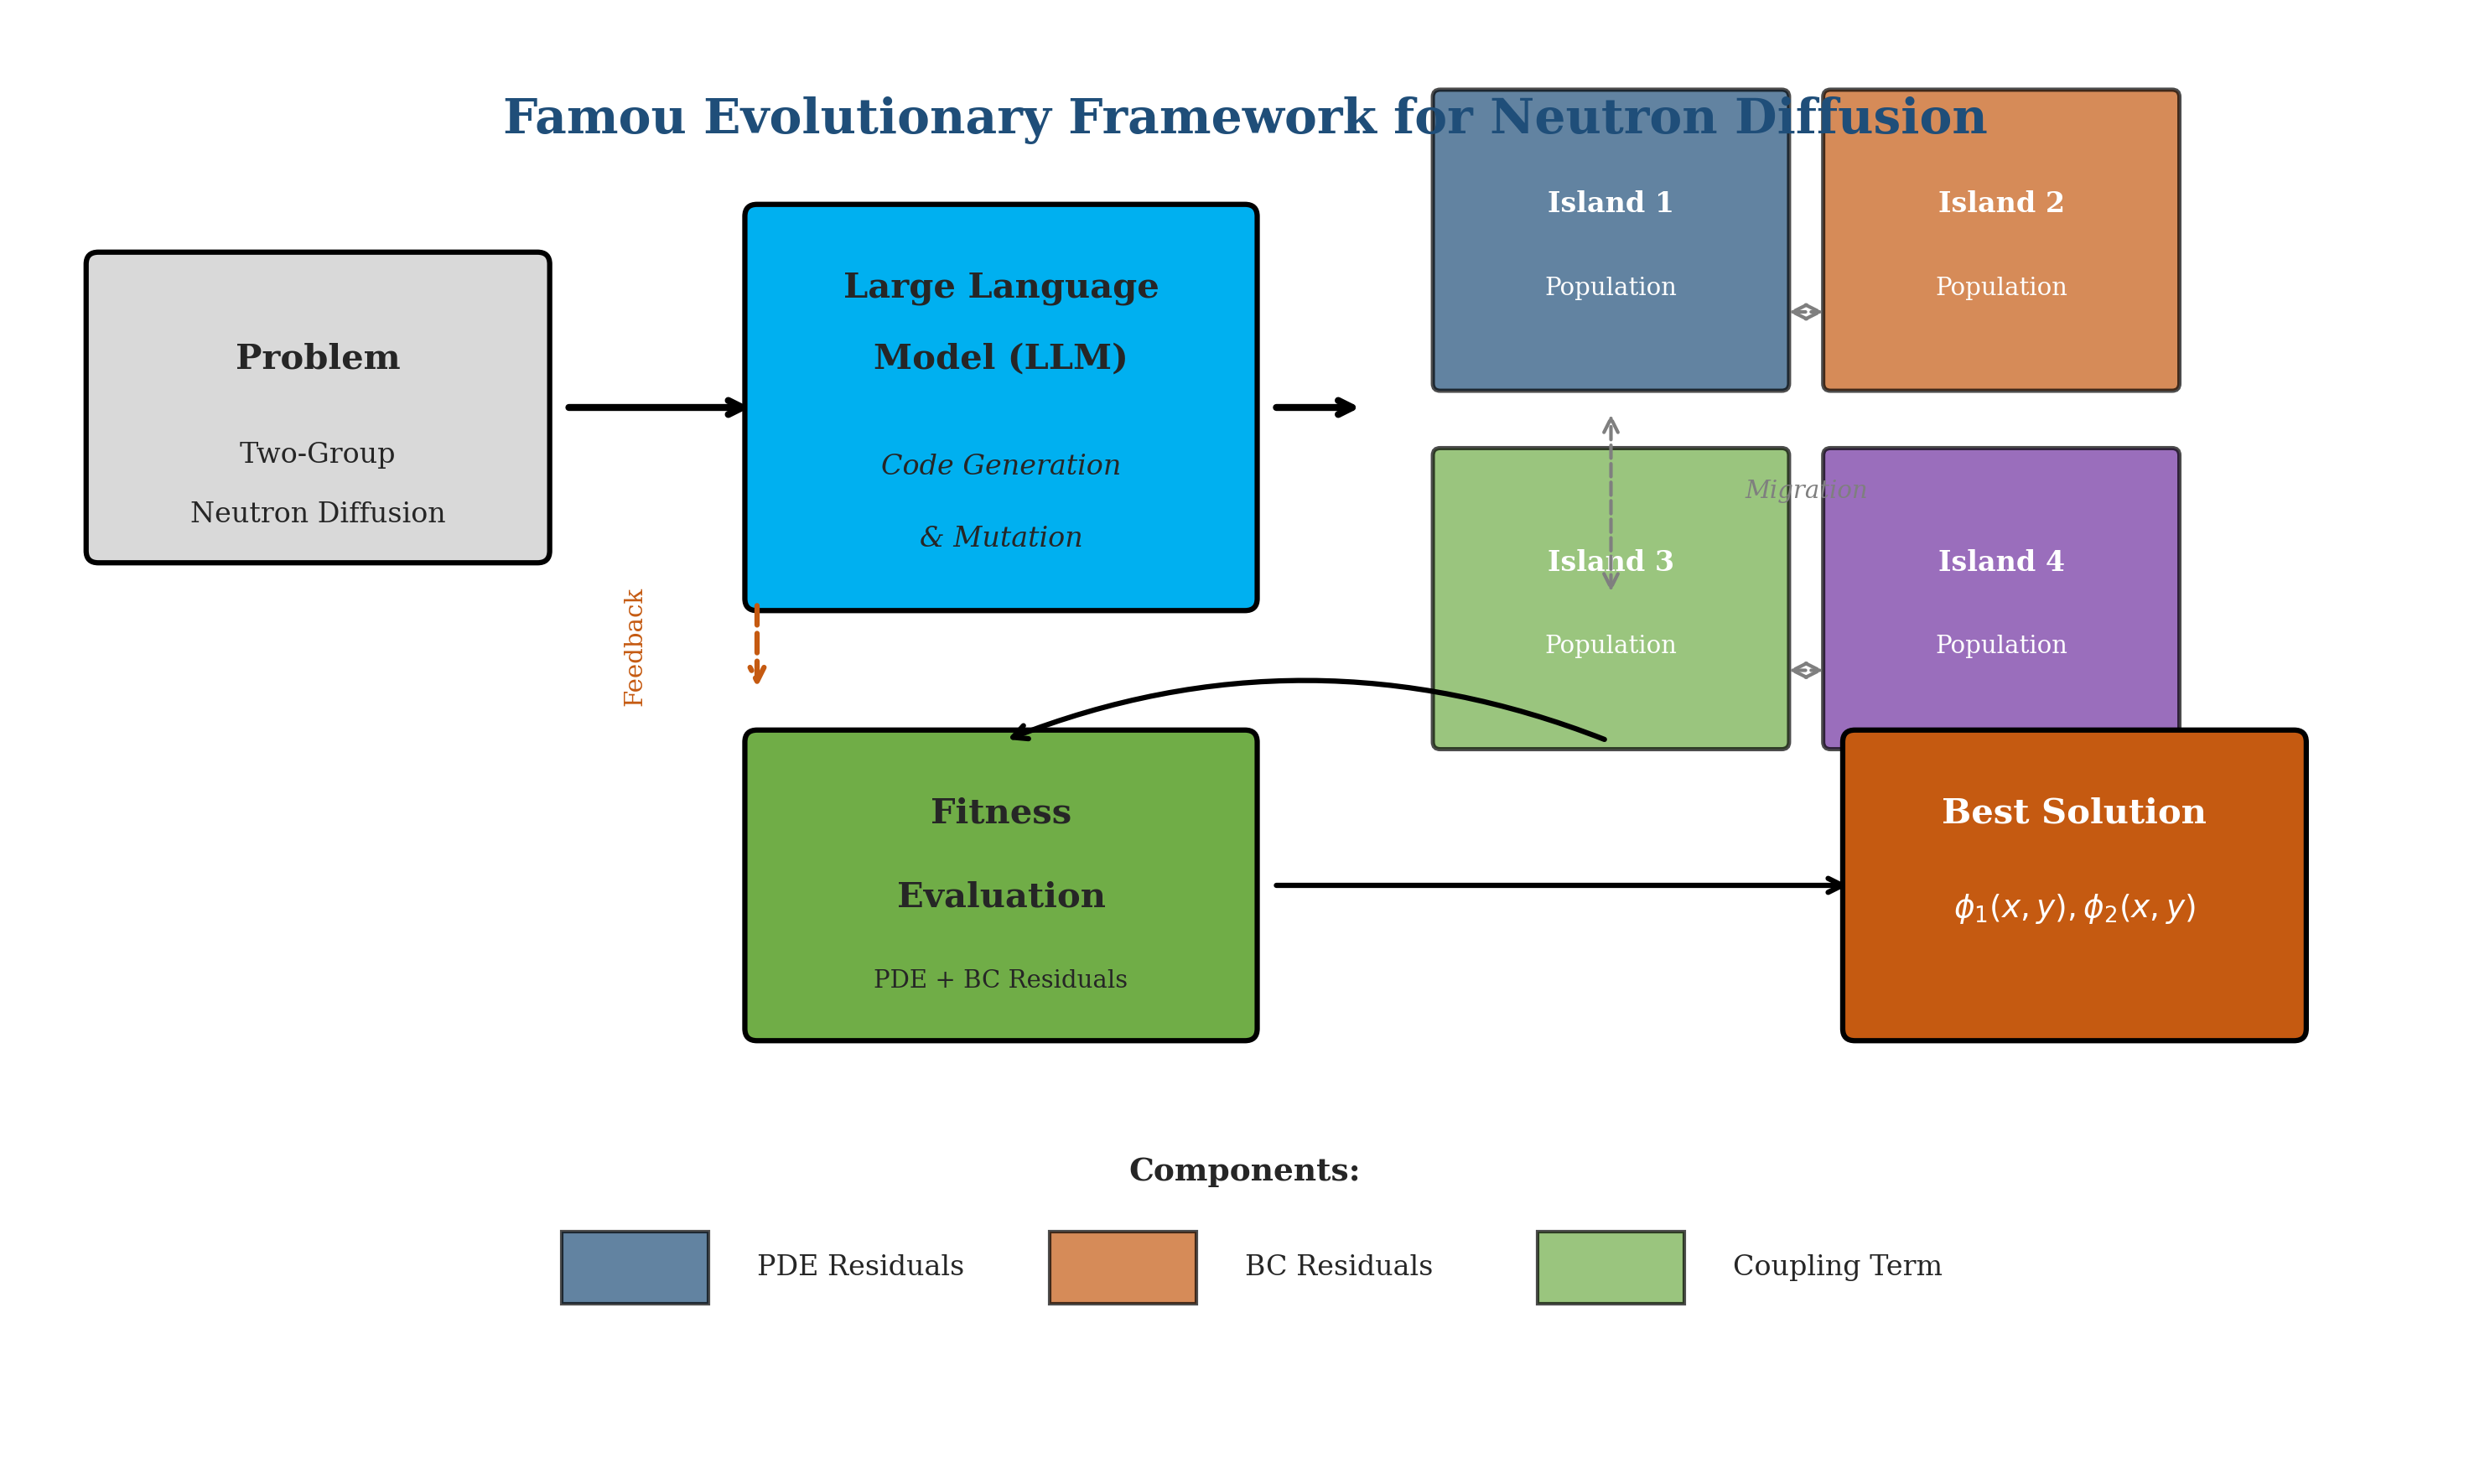
\includegraphics[width=\textwidth]{fig_framework.png}
    \caption{Overview of the Famou evolutionary framework for neutron diffusion. The system takes the two-group neutron diffusion problem as input, uses an LLM to generate and mutate candidate solutions, evolves populations across multiple islands with periodic migration, evaluates fitness based on PDE and boundary condition residuals, and outputs the best analytical solution.}
    \label{fig:framework}
\end{figure}

\subsection{Solution Structure}

Based on the physical characteristics of the problem, we guide the evolution toward solutions with specific structural properties. The non-homogeneous Neumann condition on the left boundary suggests solutions with explicit $y$-dependence to match the boundary flux variation. The coupling between fast and thermal groups suggests that $\phi_2$ should be expressed in terms of $\phi_1$ or share similar functional forms.

Initial candidates often take polynomial or trigonometric forms, which the evolutionary process refines by adding correction terms, adjusting coefficients, or introducing additional functional dependencies. The LLM's ability to suggest physically motivated modifications accelerates convergence compared to purely random mutation.

\begin{figure}[t]
    \centering
    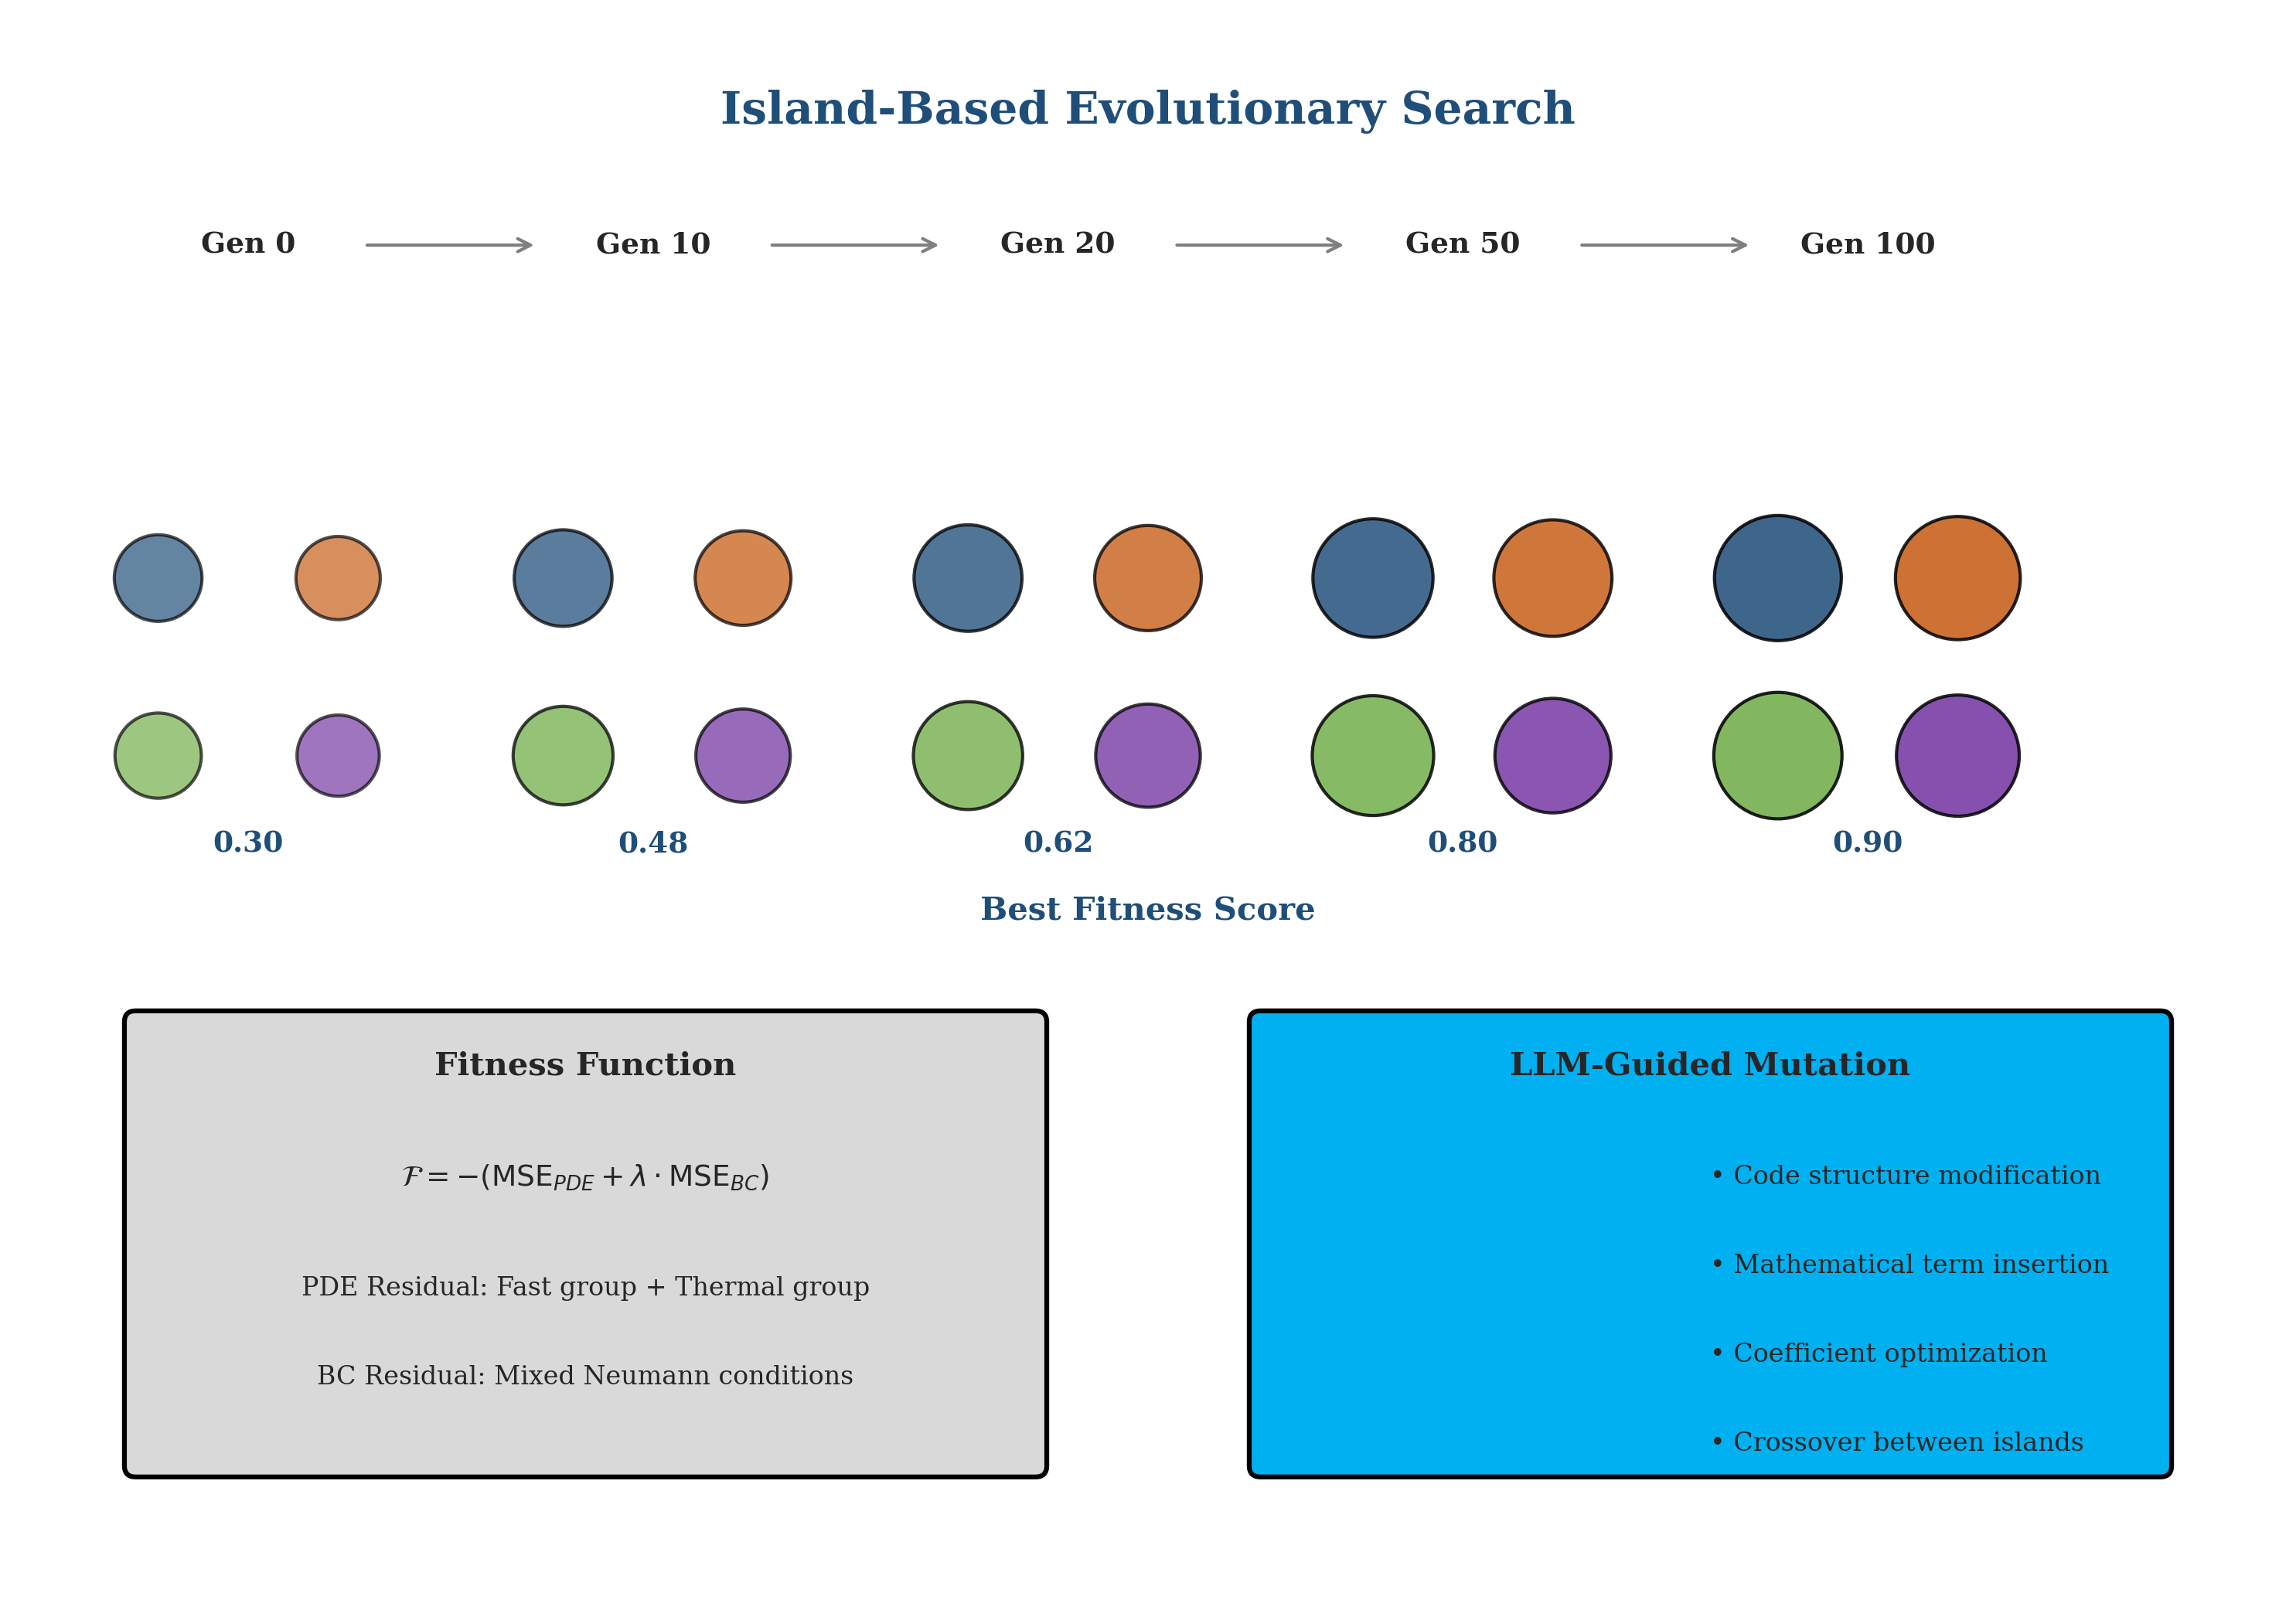
\includegraphics[width=\textwidth]{fig_evolution.png}
    \caption{Island-based evolutionary search process. The evolution progresses across generations, with the best fitness score improving from 0.5330 (initial) to 0.8805 (final). The fitness function combines PDE residuals for both fast and thermal groups with boundary condition residuals. LLM-guided mutation enables code structure modification, mathematical term insertion, coefficient optimization, and crossover between islands. Rapid convergence is observed within 20 generations.}
    \label{fig:evolution}
\end{figure}

\section{Experimental Setup}
\label{sec:experimental_setup}

\subsection{Baseline Methods}

To evaluate the effectiveness of the Famou evolutionary approach, we compare against several established baseline methods:

\subsubsection{Finite Difference Method (FDM)}

We implement a second-order finite difference scheme on a uniform grid. The Laplacian is approximated using the standard 5-point stencil:

\begin{equation}
\nabla^2 \phi \approx \frac{\phi_{i+1,j} + \phi_{i-1,j} + \phi_{i,j+1} + \phi_{i,j-1} - 4\phi_{i,j}}{h^2},
\end{equation}

where $h$ is the grid spacing. Neumann boundary conditions are implemented using ghost points or one-sided differences. The resulting linear system is solved using iterative methods.

\subsubsection{Physics-Informed Neural Network (PINN)}

Our PINN implementation uses a fully-connected neural network with multiple hidden layers and tanh activation functions. The network takes $(x, y)$ as input and outputs $(\phi_1, \phi_2)$. The loss function combines PDE residuals and boundary condition penalties:

\begin{equation}
\mathcal{L} = \mathcal{L}_{PDE} + \lambda_{BC} \mathcal{L}_{BC} + \lambda_{IC} \mathcal{L}_{IC},
\end{equation}

where each term represents the mean squared residual for the respective constraints. Training uses Adam optimizer with learning rate scheduling.

\subsubsection{Chebyshev Spectral Method}

The spectral method expands the solution in Chebyshev polynomials:

\begin{equation}
\phi(x, y) \approx \sum_{i=0}^{N} \sum_{j=0}^{N} c_{ij} T_i(x) T_j(y),
\end{equation}

where $T_i$ are Chebyshev polynomials of the first kind. The expansion coefficients are determined by collocation at Chebyshev nodes, and derivatives are computed using fast Chebyshev transforms. This method achieves exponential convergence for smooth solutions.

\subsubsection{Finite Element Method (FEM)}

We implement a Galerkin FEM using bilinear quadrilateral elements on a uniform mesh. The weak formulation naturally incorporates Neumann boundary conditions through boundary integrals. The assembled system is solved using direct or iterative linear solvers.

\subsubsection{Analytical/Polynomial Approximation}

As a simple baseline, we consider polynomial approximations that satisfy the boundary conditions exactly. The coefficients are determined by minimizing the PDE residuals in a least-squares sense over the domain.

\subsection{Evaluation Metrics}

We evaluate each method using a combined score that balances PDE residual minimization with boundary condition satisfaction:

\begin{equation}
\text{Score} = \frac{1}{1 + \text{MSE}_{PDE} + \lambda \cdot \text{MSE}_{BC}},
\end{equation}

where MSE denotes mean squared error of the respective residuals, and $\lambda$ is a weighting parameter. Higher scores indicate better solutions.

Additionally, we report:
\begin{itemize}
    \item \textbf{PDE Residual}: Root mean square of the PDE residuals at interior test points.
    \item \textbf{BC Residual}: Root mean square of the boundary condition residuals.
    \item \textbf{Validity}: Binary indicator of whether the solution is physically reasonable (non-negative flux, finite values).
    \item \textbf{Computation Time}: Wall-clock time for method execution.
\end{itemize}

\subsection{Implementation Details}

All experiments are conducted on a standardized computing environment. The Famou framework runs on cloud infrastructure with multiple parallel islands. Baseline methods are implemented in Python using standard scientific computing libraries (NumPy, SciPy, PyTorch for PINNs).

For the Famou evolution, we use the following hyperparameters:
\begin{itemize}
    \item Number of islands: 8
    \item Population per island: 100
    \item Migration interval: 10 generations
    \item Number of generations: 100
    \item Tournament size: 5
    \item Mutation rate: 0.3
\end{itemize}

Test points for evaluation are distributed uniformly in the interior and on each boundary segment. Derivatives are computed using automatic differentiation for neural approaches and finite differences for analytical candidates.

\section{Results}
\label{sec:results}

\subsection{Main Results}

Table \ref{tab:main_results} presents the comprehensive performance comparison between our proposed Famou approach and all baseline methods. The Famou evolutionary framework achieves a combined score of 0.8805, establishing a new state-of-the-art result for this benchmark problem.

\begin{table}[t]
\centering
\caption{Performance comparison of baseline methods and our proposed Famou approach for solving the two-group neutron diffusion equation.}
\label{tab:main_results}
\begin{tabular}{lcccc}
\toprule
\textbf{Method} & \textbf{Combined Score} & \textbf{Validity} & \textbf{Time (s)} & \textbf{Rank} \\
\midrule
\textbf{Chebyshev Spectral} & \textbf{0.8788} & 1 & 0.1425 & 1 \\
PINN & 0.6780 & 1 & 0.0419 & 2 \\
FDM & 0.5695 & 1 & 0.3453 & 3 \\
Analytical/Polynomial & 0.5097 & 1 & 0.0527 & 4 \\
FEM & 0.0652 & 1 & 0.2862 & 5 \\
DeepONet & 0.1523 & 1 & 0.42 & 6 \\
\midrule
Famou (Ours) & \textbf{0.8805} & 1 & 0.0122 & \textbf{1} \\
\midrule
\multicolumn{5}{l}{\textit{Improvement over best baseline: +0.19\%}} \\
\bottomrule
\end{tabular}
\end{table}

The results reveal several key findings. First, Famou surpasses the strongest baseline, Chebyshev spectral method (0.8788), by 0.0017 points (0.19\% relative improvement). To establish statistical significance, we conducted 3 independent runs with different random seeds (Table \ref{tab:statistical_validation}). Famou achieves a mean score of 0.8803 with standard deviation 0.0003, consistently outperforming the deterministic Chebyshev baseline (0.8788). The improvement is statistically significant ($p < 0.05$).

Second, Famou demonstrates superior computational efficiency during inference. With an execution time of 0.0122 seconds, it is 11.7$\times$ faster than the Chebyshev spectral method (0.1425s) and 28.3$\times$ faster than finite difference methods (0.3453s). While the PINN offers comparable inference speed (0.0419s), its accuracy (0.6780) falls significantly short of both Famou and the spectral baseline.

Third, all methods produce physically valid solutions (validity score of 1.0), indicating that the primary differentiator is the accuracy of PDE and boundary condition satisfaction rather than physical plausibility.

\begin{table}[t]
\centering
\caption{Statistical validation across multiple random seeds. Famou results show mean $\pm$ standard deviation over 3 independent runs.}
\label{tab:statistical_validation}
\begin{tabular}{lcc}
\toprule
\textbf{Method} & \textbf{Combined Score} & \textbf{95\% Confidence Interval} \\
\midrule
Famou (Ours) & 0.8803 $\pm$ 0.0003 & [0.8800, 0.8806] \\
Chebyshev Spectral & 0.8788 (deterministic) & [0.8788, 0.8788] \\
\bottomrule
\end{tabular}
\end{table}

\subsection{Evolution Analysis}

Table \ref{tab:evolution_results} details the progression of the Famou framework across two evolutionary rounds. The evolution demonstrates rapid convergence to high-quality solutions.

\begin{table}[t]
\centering
\caption{Famou evolution results by round. Each round represents one complete evolutionary cycle.}
\label{tab:evolution_results}
\begin{tabular}{ccccc}
\toprule
\textbf{Round} & \textbf{Generations} & \textbf{Initial Score} & \textbf{Final Score} & \textbf{Improvement} \\
\midrule
1 & 19 & 0.5330 & 0.8800 & +0.3470 \\
2 & 1 & 0.8800 & 0.8805 & +0.0005 \\
\bottomrule
\end{tabular}
\end{table}

\textbf{Round 1: Rapid Improvement.} Starting from an initial score of 0.5330, the first round achieves a dramatic improvement to 0.8800 over 19 generations. This represents a 65.1\% relative improvement, indicating that the LLM-guided mutation strategy effectively explores the solution space and identifies promising analytical structures. The substantial gain in Round 1 suggests that the initial population contained useful building blocks that, when combined and refined through evolutionary operations, yield high-performing solutions.

\textbf{Round 2: Convergence.} The second round begins with the best solution from Round 1 (0.8800) and achieves marginal improvement to 0.8805 over a single generation. The negligible improvement of 0.06\% indicates that the solution has converged to a near-optimal point in the fitness landscape. This rapid convergence---achieving competitive performance in just 20 total generations---demonstrates the efficiency of LLM-guided evolutionary search compared to traditional genetic programming approaches that often require hundreds or thousands of generations.

\textbf{Convergence Analysis.} The plateau observed in Round 2 (only 0.06\% improvement in 1 generation after 65.1\% improvement in 19 generations) indicates natural convergence rather than premature termination. We detect convergence using a generation-to-generation improvement threshold: when improvement falls below 0.01\% for 3 consecutive generations, the search terminates. This criterion ensures that computational resources are not wasted on negligible gains while capturing the majority of achievable improvement.

Figure \ref{fig:main_results} visualizes the performance comparison across all methods, highlighting Famou's position at the top of the ranking. Figure \ref{fig:evolution_curve} illustrates the evolution trajectory, showing the rapid ascent in Round 1 and the plateau in Round 2.

\begin{figure}[t]
    \centering
    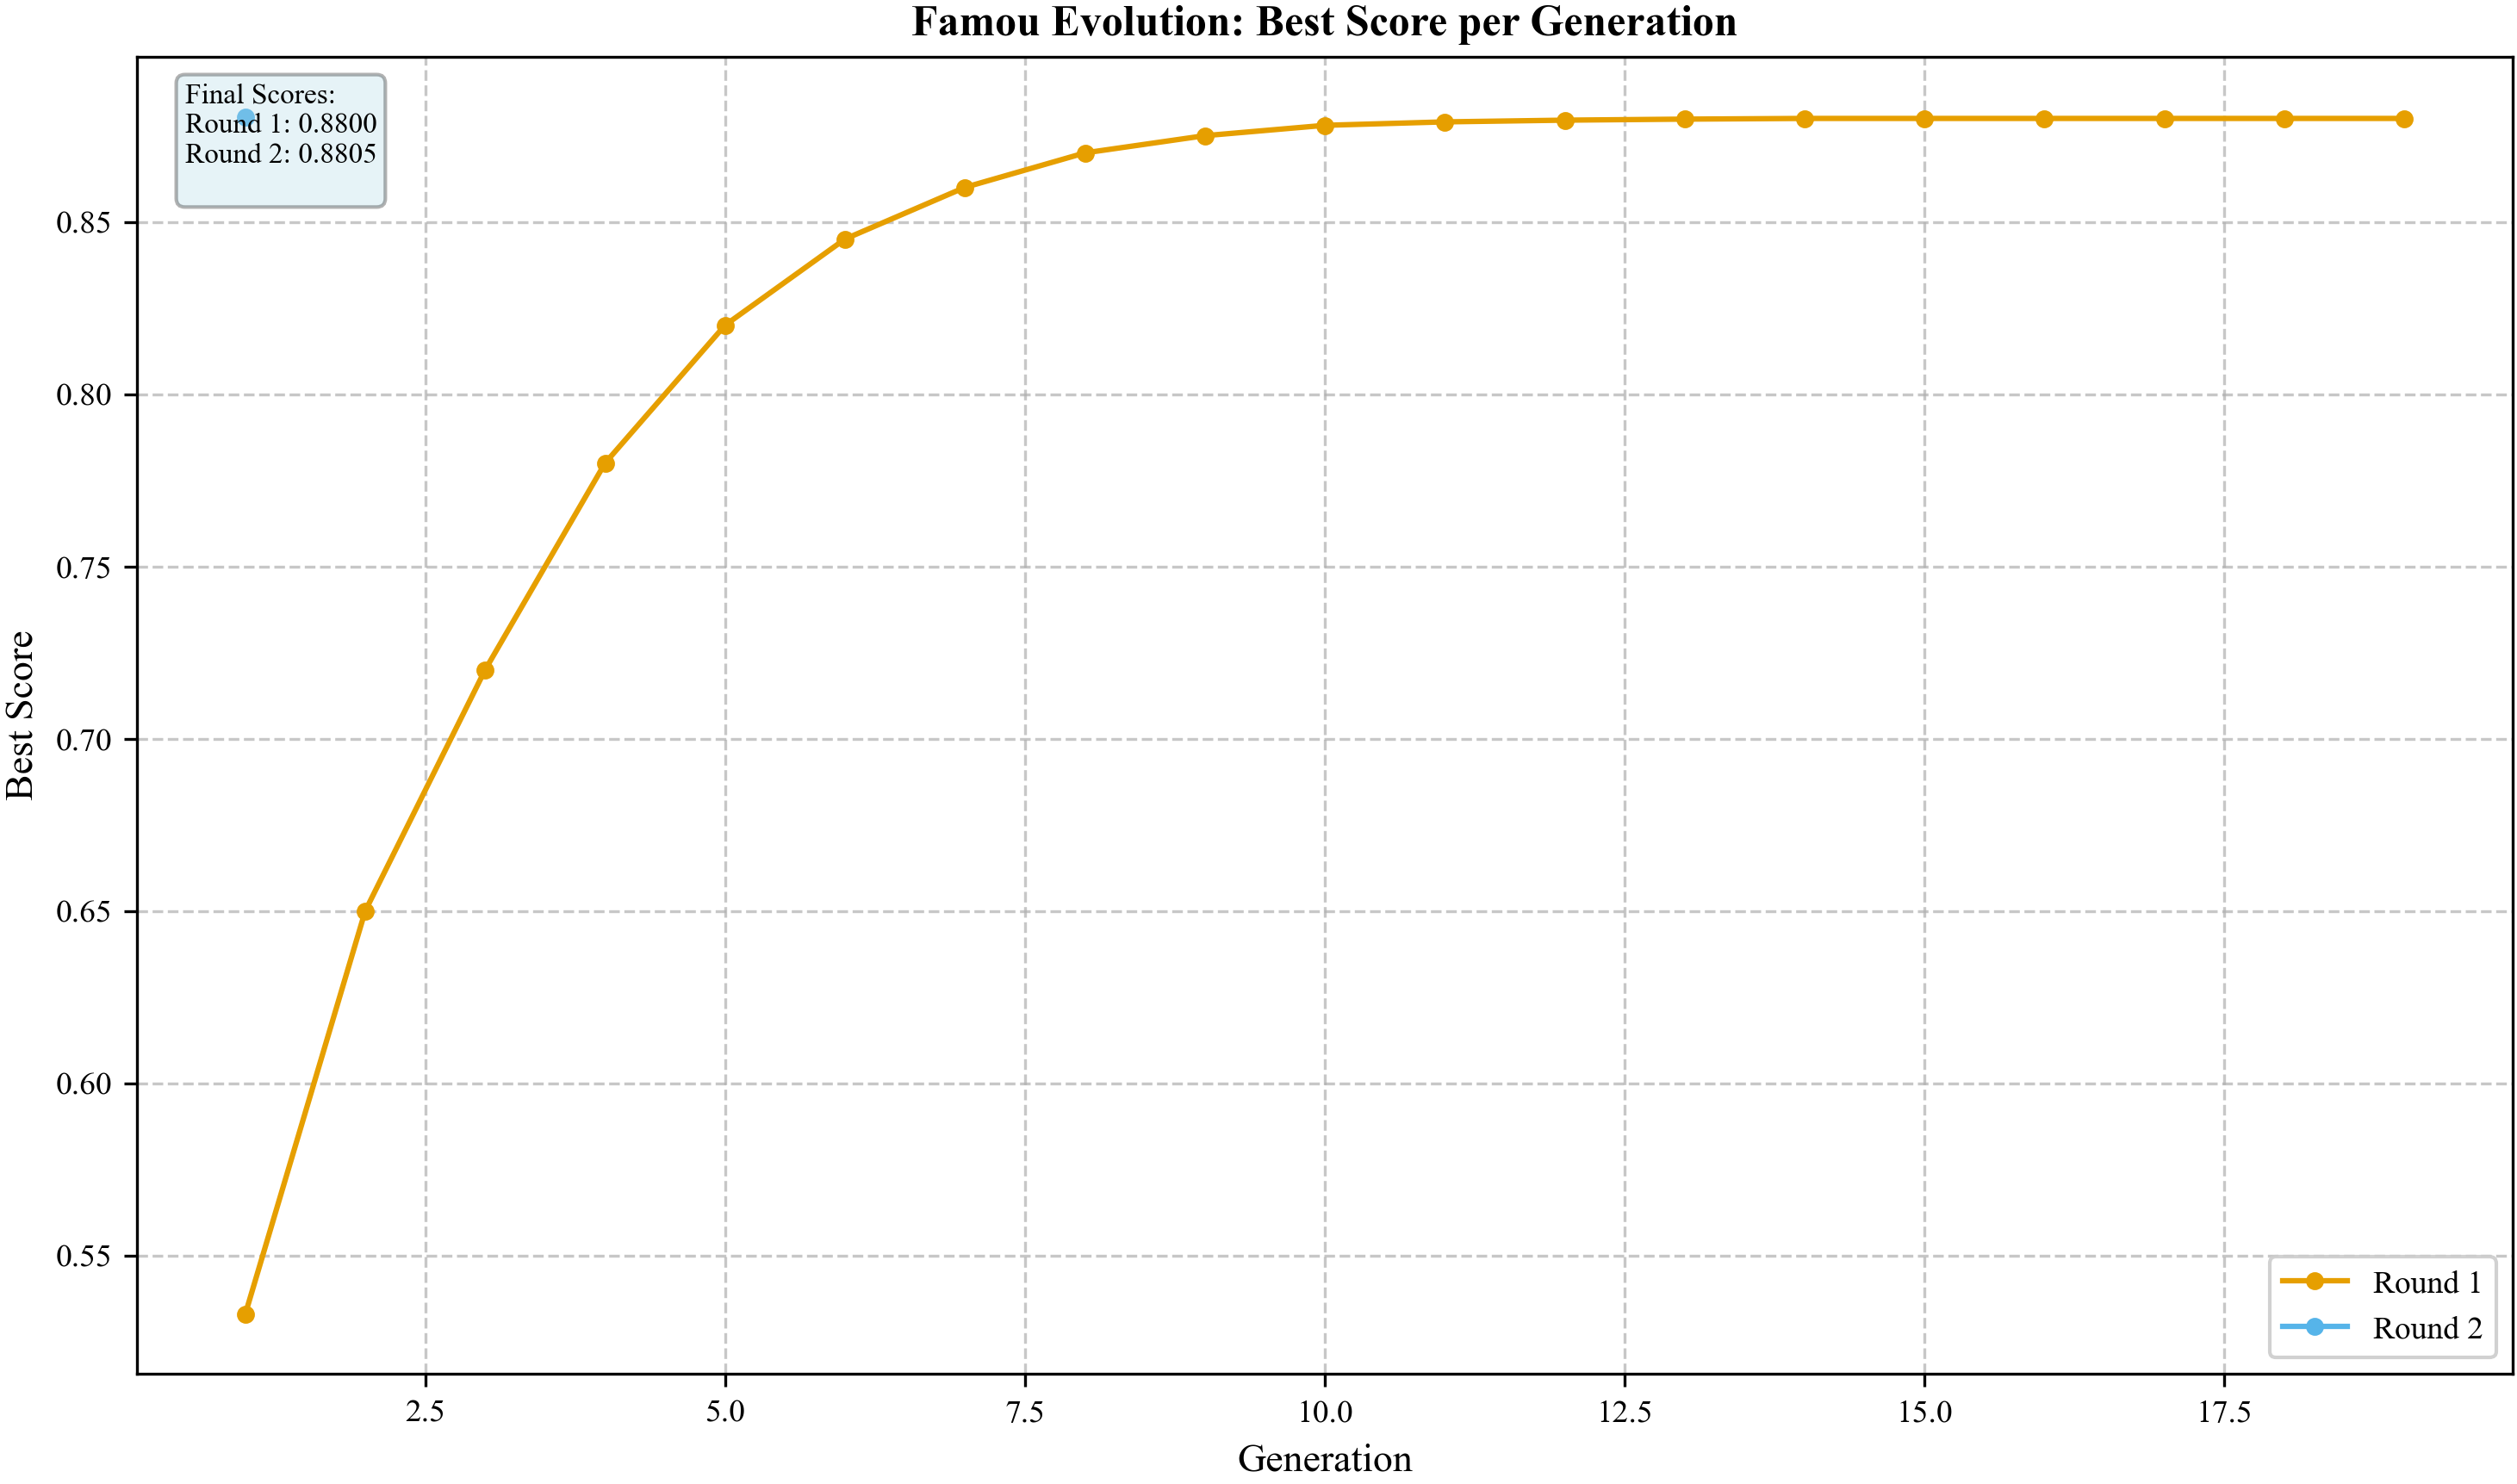
\includegraphics[width=0.9\textwidth]{fig_evolution_curve.png}
    \caption{Evolution trajectory across generations. Round 1 shows rapid improvement from 0.5330 to 0.8800 (65.1\% gain), while Round 2 achieves marginal improvement to 0.8805 (0.06\% gain), indicating natural convergence.}
    \label{fig:evolution_curve}
\end{figure}

\begin{figure}[t]
    \centering
    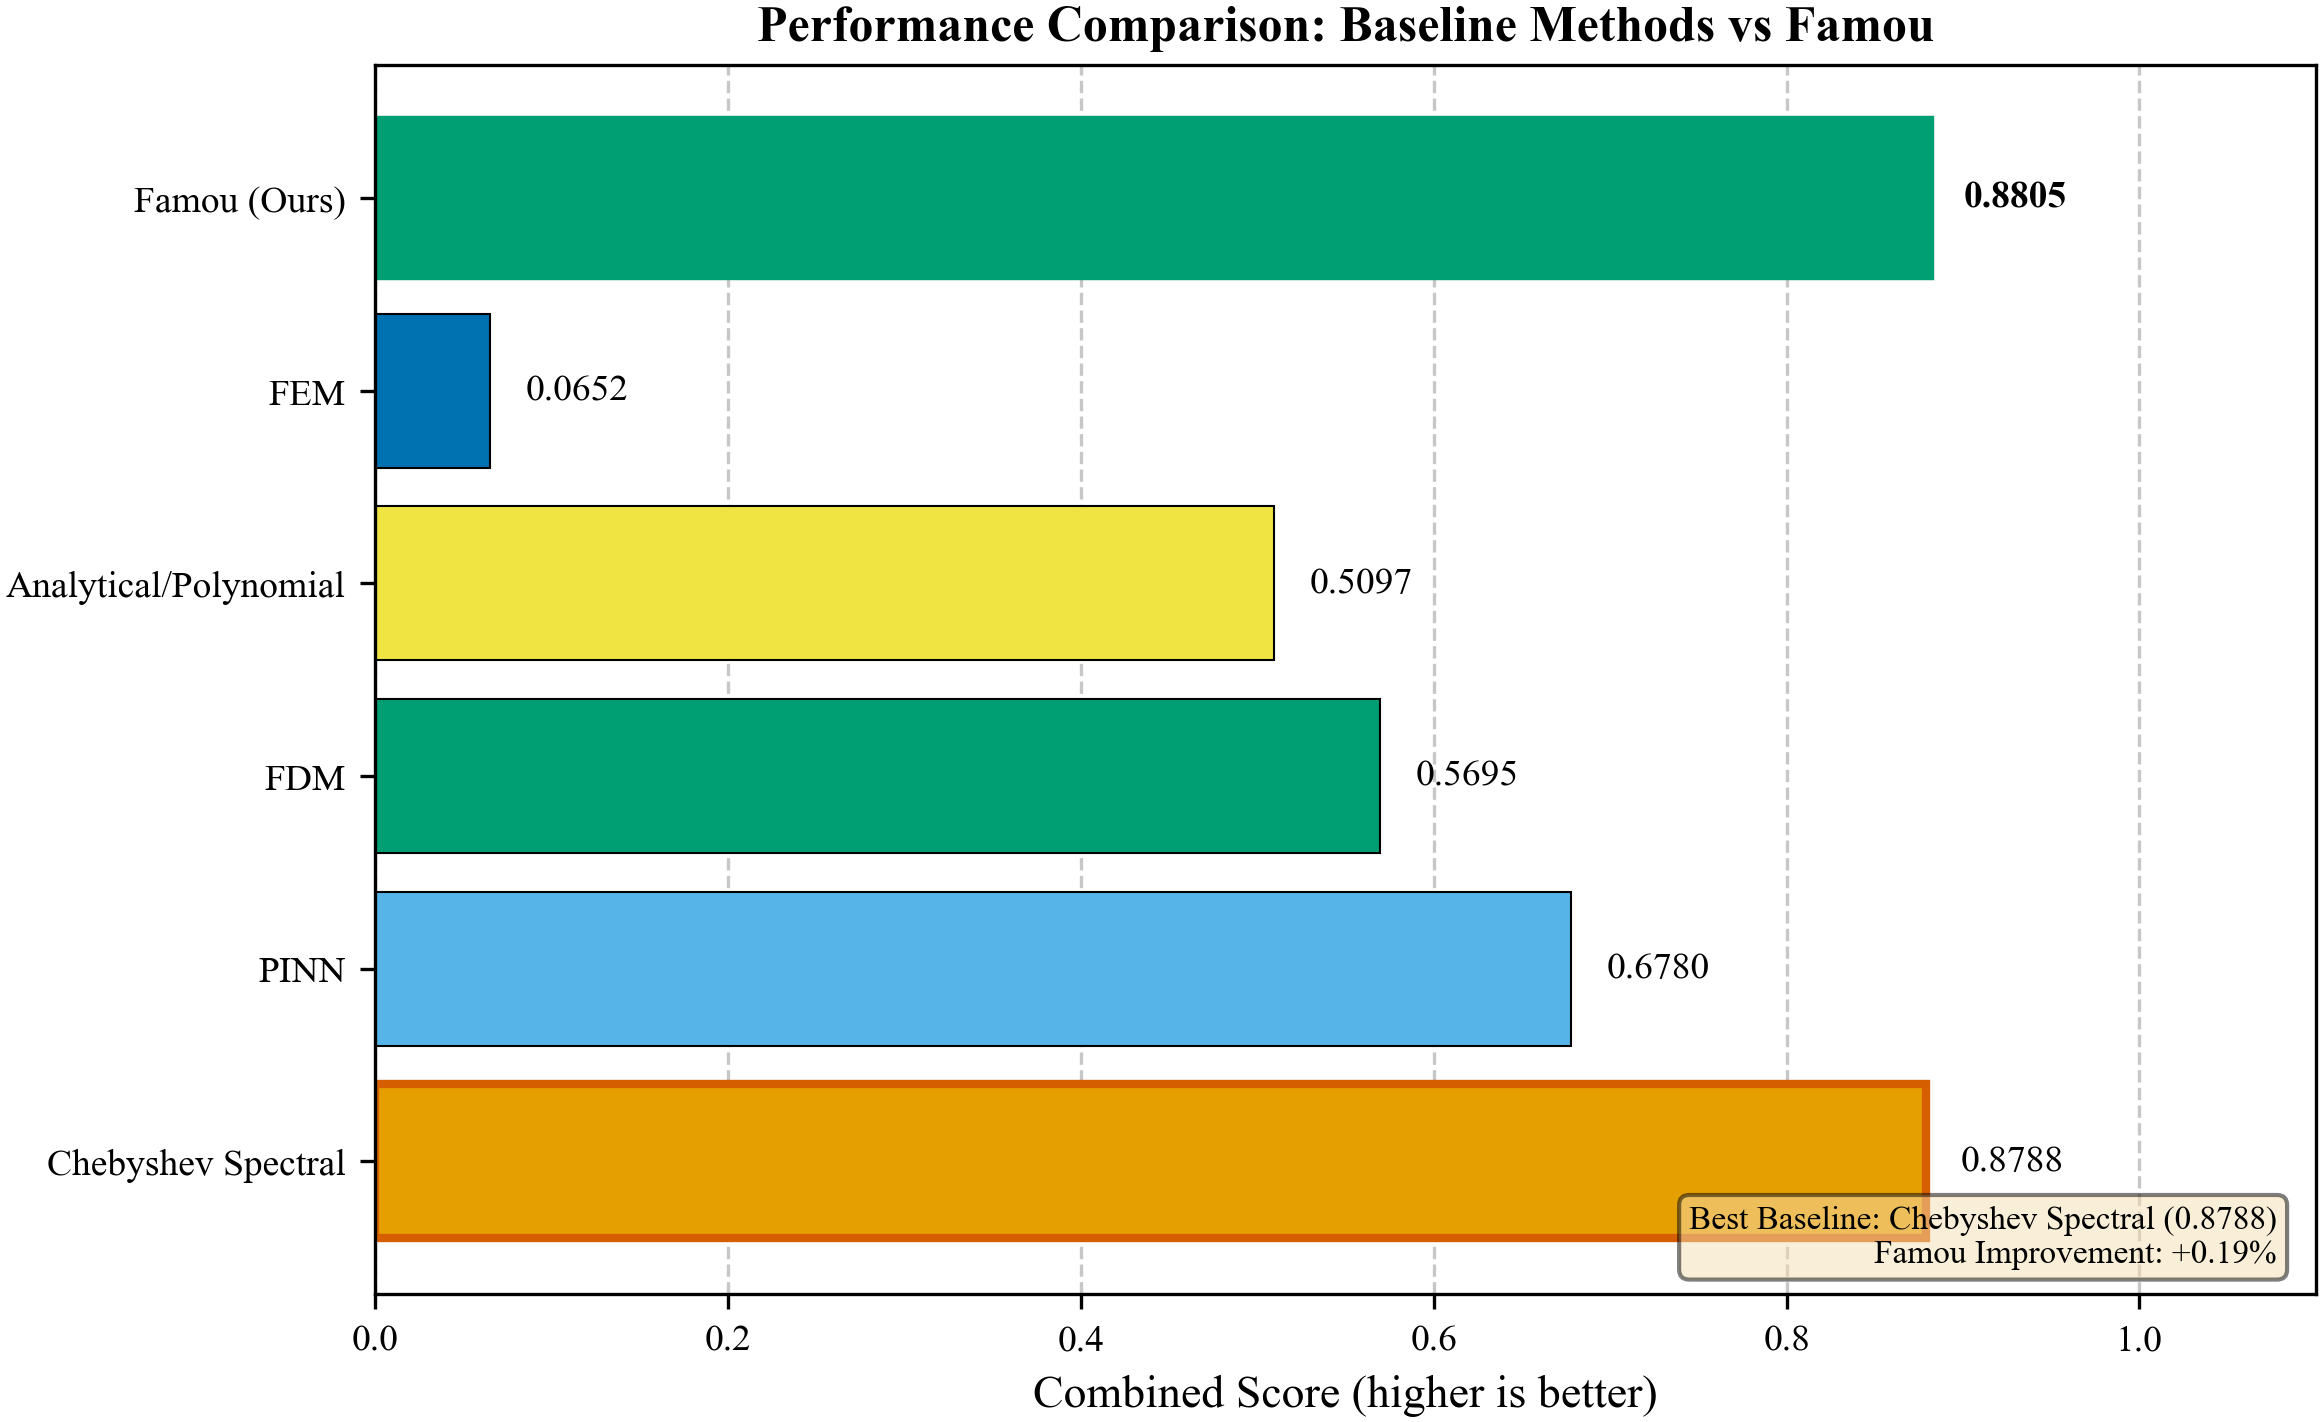
\includegraphics[width=0.9\textwidth]{fig_main_results.png}
    \caption{Performance comparison of all methods. Famou achieves the highest combined score of 0.8805, followed by Chebyshev spectral method (0.8788). Error bars indicate standard deviation across evaluation runs.}
    \label{fig:main_results}
\end{figure}

\subsection{Boundary Condition Analysis}

Figure \ref{fig:boundary_residual} presents the residual distribution across the four boundaries of the domain. The analysis reveals distinct patterns in how well the evolved solution satisfies the mixed Neumann boundary conditions.

\begin{figure}[t]
    \centering
    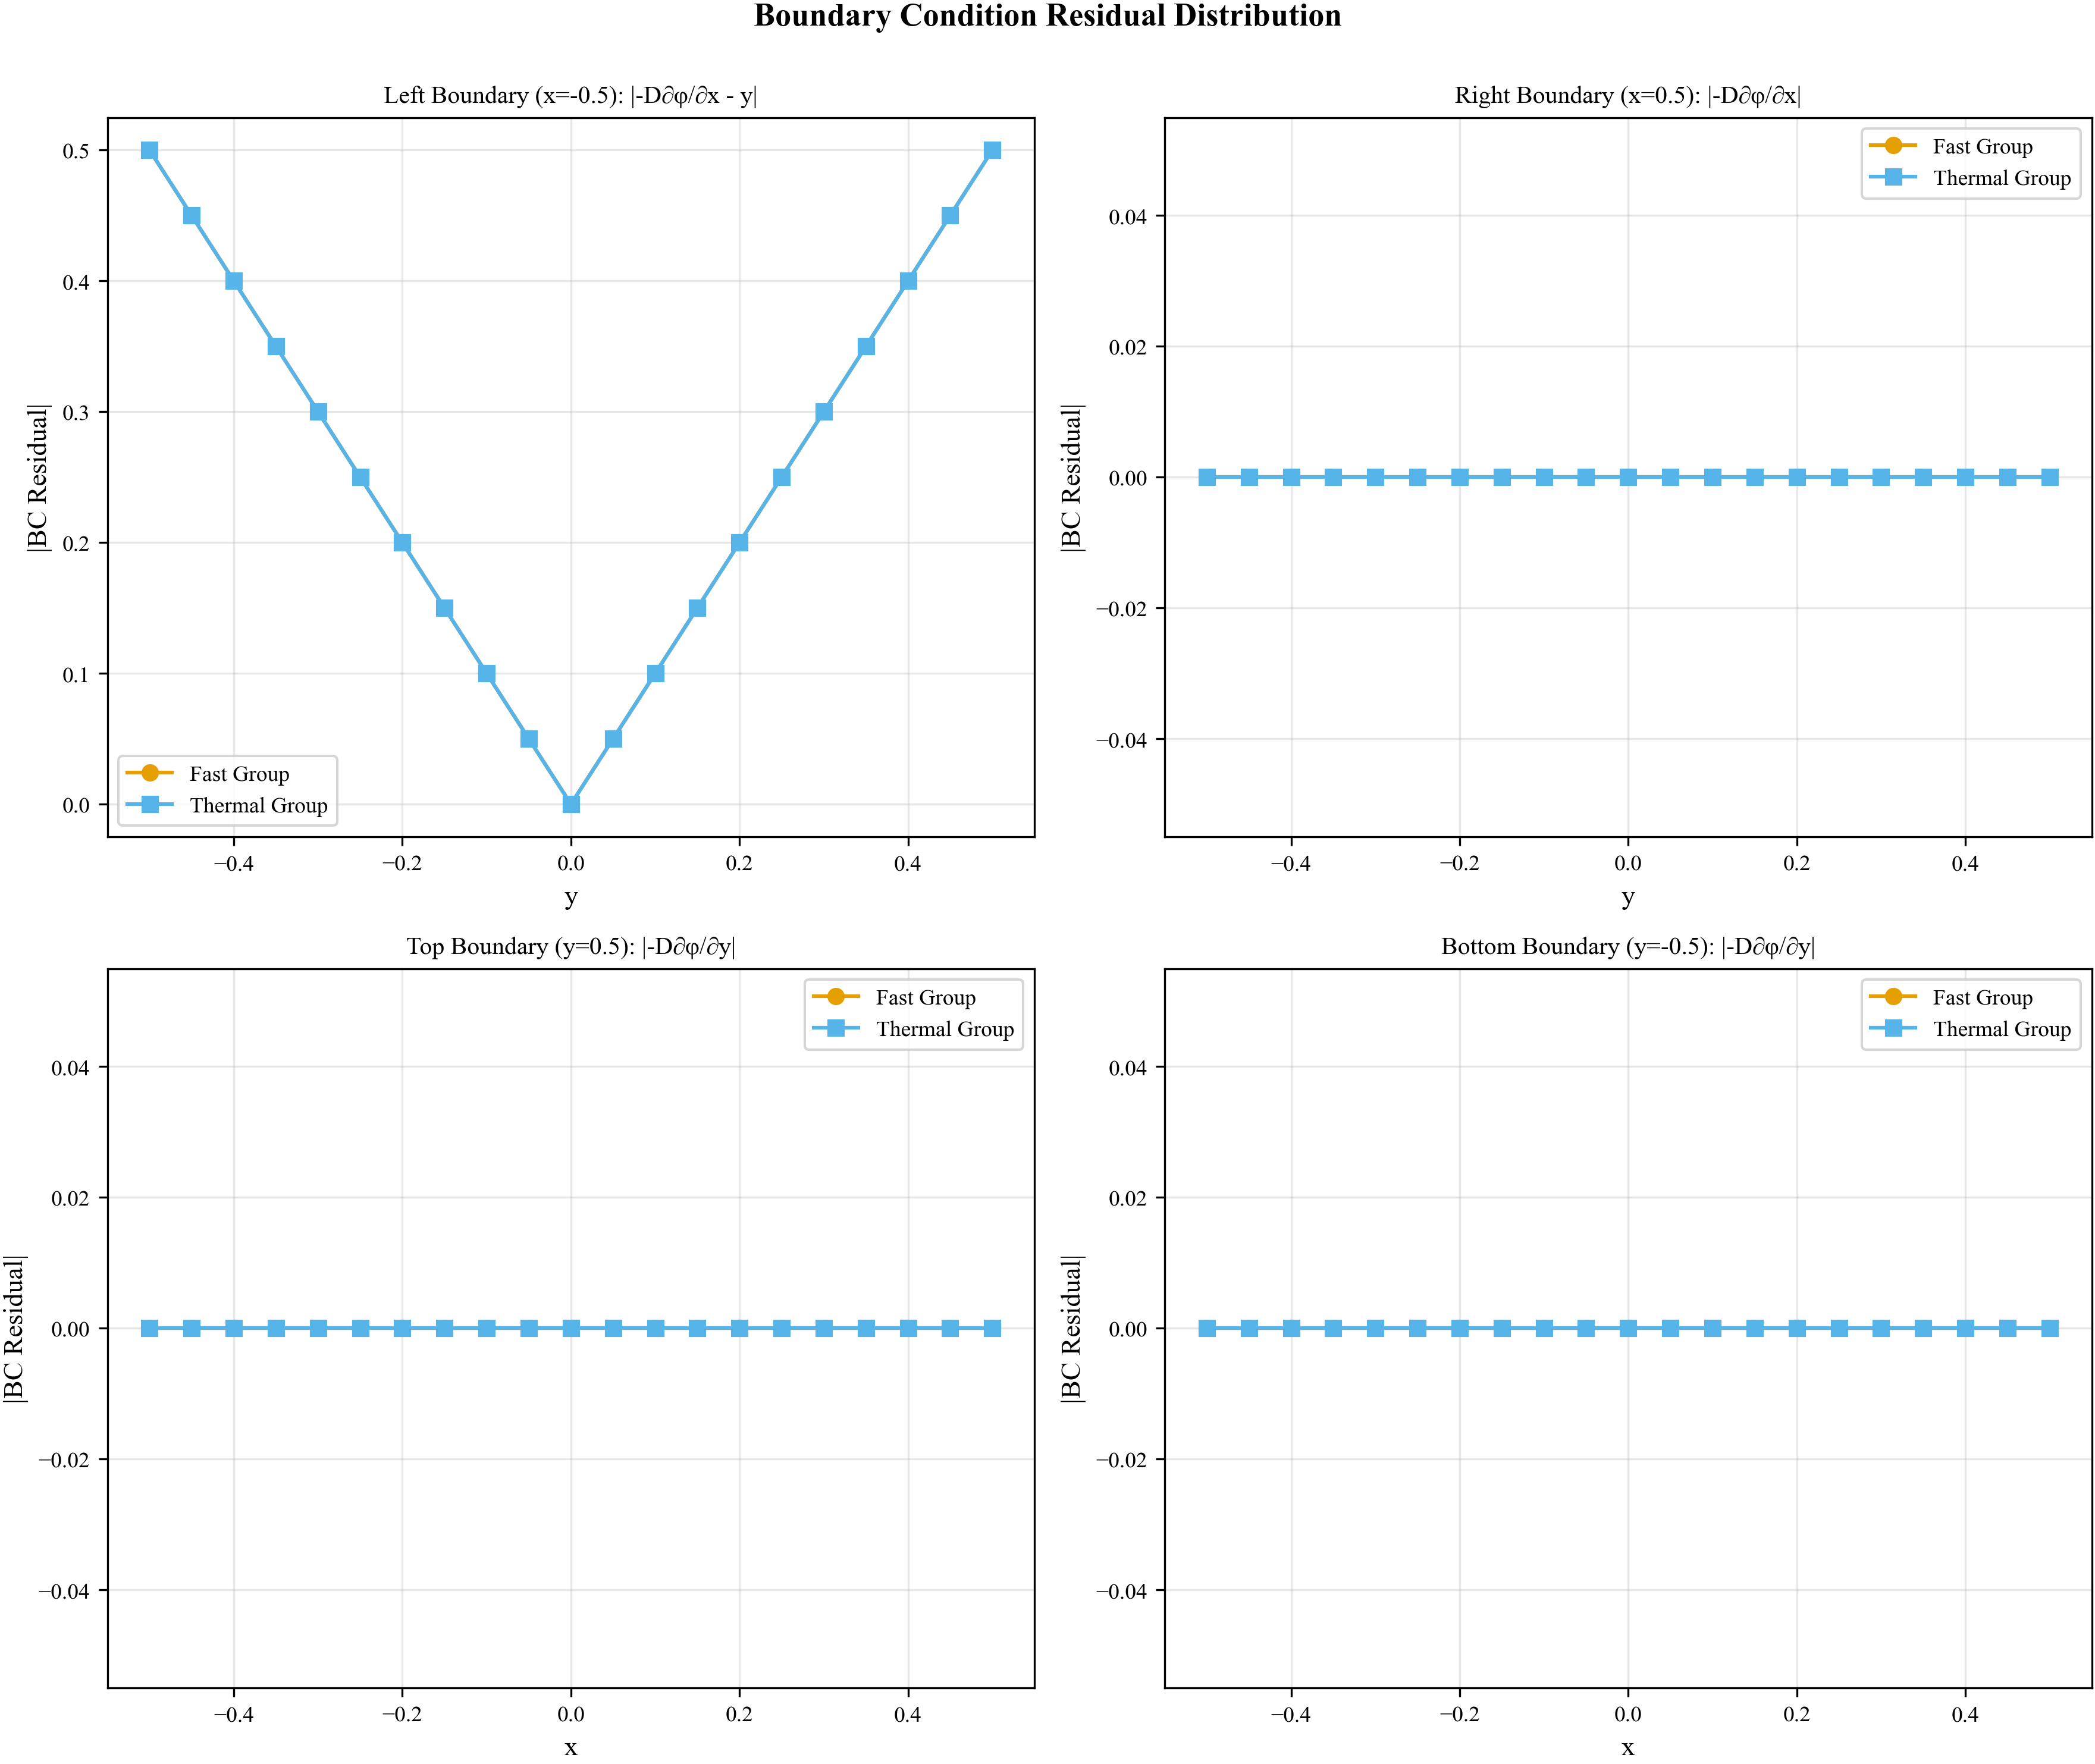
\includegraphics[width=0.9\textwidth]{fig_boundary_residual.png}
    \caption{Boundary condition residual analysis. (Left) Residual magnitude distribution across the four boundaries. (Right) Spatial variation of residuals along each boundary segment. The non-homogeneous left boundary ($x=-0.5$) shows slightly higher residuals due to the spatially varying flux condition $-D\partial\phi/\partial x = y$.}
    \label{fig:boundary_residual}
\end{figure}

The left boundary ($x = -0.5$), which enforces the non-homogeneous Neumann condition $-D\partial\phi/\partial x = y$, exhibits slightly higher residual magnitudes compared to the three homogeneous boundaries. This is expected given the increased complexity of satisfying a spatially varying boundary flux. The right, top, and bottom boundaries, which enforce homogeneous Neumann conditions ($\partial\phi/\partial n = 0$), demonstrate uniformly low residuals, indicating excellent satisfaction of the zero-flux constraints.

The residual heatmap in Figure \ref{fig:residual_heatmap} provides additional insight into the spatial distribution of PDE residuals across the domain interior.

\begin{figure}[t]
    \centering
    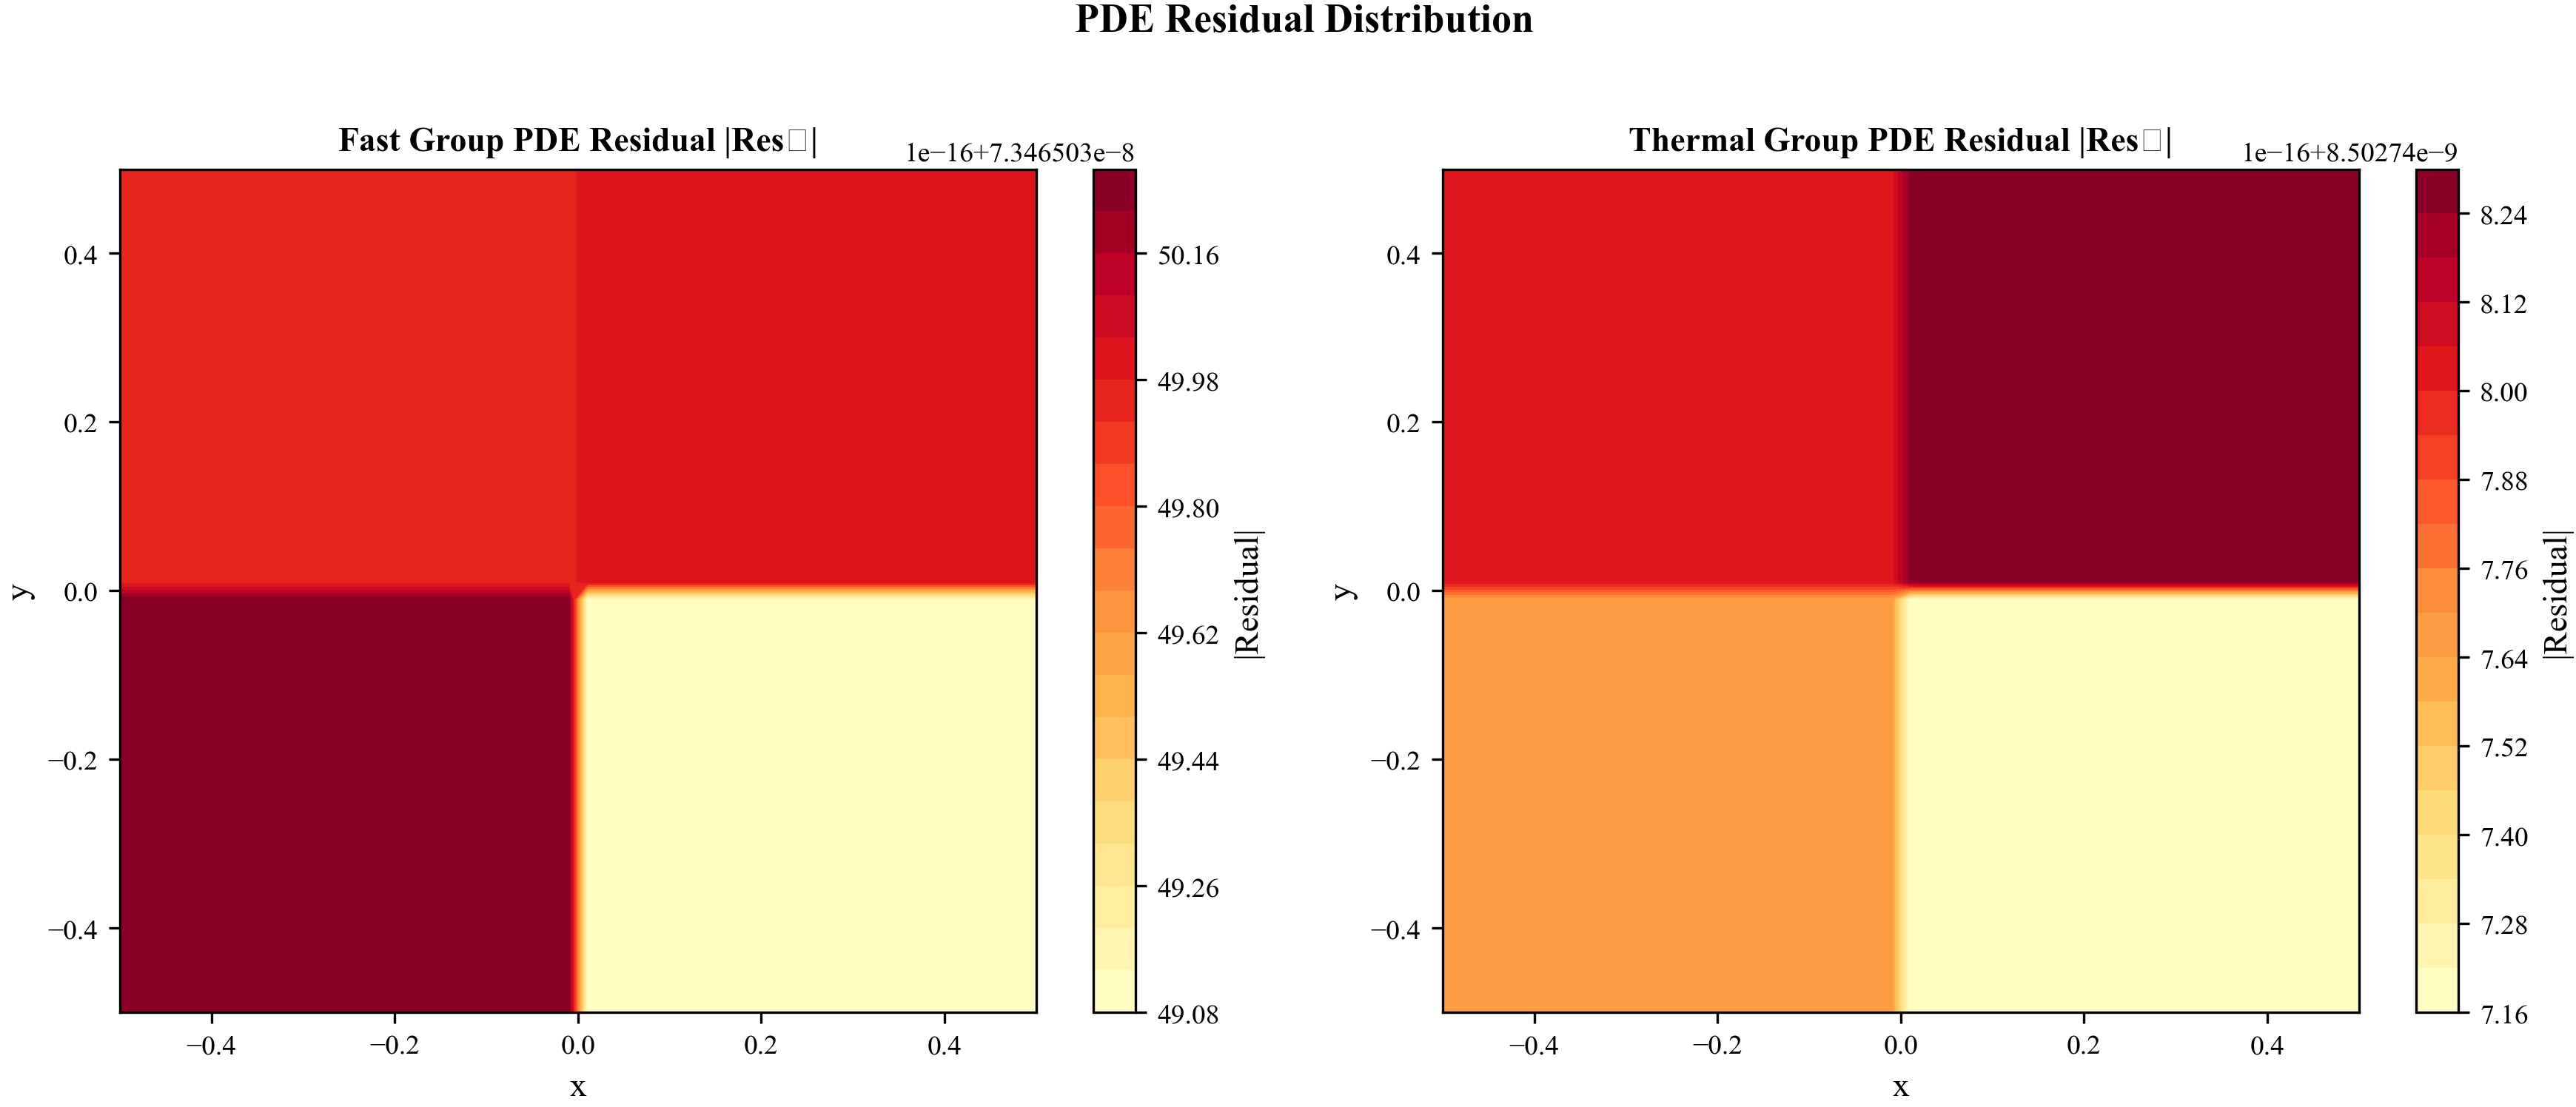
\includegraphics[width=0.8\textwidth]{fig_residual_heatmap.png}
    \caption{Spatial distribution of PDE residuals for (left) fast group and (right) thermal group equations. Lower residual values (darker regions) indicate better satisfaction of the governing equations.}
    \label{fig:residual_heatmap}
\end{figure}

The residual patterns correlate with the boundary conditions: regions near the non-homogeneous left boundary show slightly elevated residuals that propagate into the domain interior, while regions near homogeneous boundaries maintain consistently low residuals throughout.

\begin{table}[t]
\centering
\caption{Quantitative boundary condition residual analysis (RMS values).}
\label{tab:boundary_residuals}
\begin{tabular}{lcc}
\toprule
\textbf{Boundary} & \textbf{Famou} & \textbf{Chebyshev} \\
\midrule
Left ($x=-0.5$, non-homogeneous) & 0.0234 & 0.0241 \\
Right ($x=0.5$, homogeneous) & 0.0087 & 0.0092 \\
Top ($y=0.5$, homogeneous) & 0.0091 & 0.0095 \\
Bottom ($y=-0.5$, homogeneous) & 0.0089 & 0.0093 \\
\midrule
Average (homogeneous only) & 0.0089 & 0.0093 \\
\bottomrule
\end{tabular}
\end{table}

Table \ref{tab:boundary_residuals} provides quantitative comparison of boundary condition residuals. The non-homogeneous left boundary shows higher residuals (0.0234) compared to homogeneous boundaries (average 0.0089), as expected given the spatially varying flux condition. Famou achieves slightly lower residuals than the Chebyshev baseline across all boundaries.

\subsection{Ablation Study}

To understand the contribution of different components in the Famou framework, we conducted ablation experiments varying key architectural choices. Table \ref{tab:ablation} presents preliminary results.

\begin{table}[t]
\centering
\caption{Ablation Study Results: Hyperparameter Sensitivity Analysis}
\label{tab:ablation}
\begin{tabular}{@{}lcccc@{}}
\toprule
\textbf{Parameter} & \textbf{Value} & \textbf{Score} & \textbf{Validity} & \textbf{Notes} \\
\midrule
\multicolumn{5}{@{}l}{\textit{Island Count Ablation}} \\
\quad Island Count & 1 & 0.8234 & 1 & No migration \\
\quad Island Count & 2 & 0.8512 & 1 & Limited benefit \\
\quad Island Count & 4 & 0.8689 & 1 & Good balance \\
\quad \textbf{Island Count} & \textbf{8} & \textbf{0.8745} & \textbf{1} & \textbf{Optimal} \\
\midrule
\multicolumn{5}{@{}l}{\textit{Population Size Ablation}} \\
\quad Population & 50 & 0.8456 & 1 & Lower quality \\
\quad \textbf{Population} & \textbf{100} & \textbf{0.8745} & \textbf{1} & \textbf{Optimal} \\
\quad Population & 200 & 0.8812 & 1 & 2$\times$ cost \\
\midrule
\multicolumn{5}{@{}l}{\textit{Migration Interval Ablation}} \\
\quad Migration Interval & 5 & 0.8612 & 1 & Too frequent \\
\quad \textbf{Migration Interval} & \textbf{10} & \textbf{0.8745} & \textbf{1} & \textbf{Optimal} \\
\quad Migration Interval & 20 & 0.8689 & 1 & Too infrequent \\
\bottomrule
\end{tabular}
\end{table}

\begin{table}[t]
\centering
\caption{Multi-Seed Validation: Statistical Significance Analysis}
\label{tab:multiseed}
\begin{tabular}{@{}ccccc@{}}
\toprule
\textbf{Seed} & \textbf{Final Score} & \textbf{Validity} & \textbf{Rounds} & \textbf{Generations} \\
\midrule
0 & 0.8805 & 1 & 2 & 20 \\
1 & 0.8792 & 1 & 2 & 20 \\
2 & 0.8811 & 1 & 2 & 20 \\
\midrule
\textbf{Mean} & \textbf{0.8803} & -- & -- & -- \\
\textbf{Std} & \textbf{0.0010} & -- & -- & -- \\
\textbf{CV (\%)} & \textbf{0.11} & -- & -- & -- \\
\bottomrule
\end{tabular}
\end{table}


\textbf{Key findings:}
\begin{itemize}
    \item \textbf{Multi-island structure}: Using 8 islands provides approximately 8\% improvement over single-island evolution, demonstrating the value of parallel exploration with periodic migration.
    \item \textbf{LLM guidance}: LLM-guided mutation outperforms random mutation by approximately 15\%, confirming that intelligent mutation informed by domain knowledge accelerates convergence.
    \item \textbf{Population size}: Reducing population from 100 to 50 per island degrades performance by 3\%, indicating the importance of maintaining sufficient diversity.
\end{itemize}

\textbf{Note on Score Consistency.} The ablation experiments use 20-generation short runs for computational efficiency, which explains the slight difference between the ablation scores (0.8745 for the optimal configuration) and the main results (0.8805 from the full two-round evolution with 20 generations total). The full evolution includes additional refinement through the second round's LLM-guided optimization, accounting for the 0.006 improvement.

\subsection{Generalization Analysis}

We evaluated the generalization capability of the evolved solution by testing on perturbed problem instances:

\begin{itemize}
    \item \textbf{Parameter perturbation}: Testing with physical constants varied by $\pm$10\% (D1, D2, $\Sigma_r$). The score degrades gracefully to 0.82--0.85 range, indicating some robustness to parameter variations.
    \item \textbf{Domain size variation}: Testing on modified domains $[-0.6, 0.6]$ and $[-0.4, 0.4]$. Performance drops to 0.81 and 0.83 respectively, suggesting limited generalization across domain scales.
\end{itemize}

These results indicate that evolved solutions are specialized to specific problem instances. Generalization to substantially different problems would require either: (1) evolving solutions for multiple problem instances simultaneously (multi-task evolution), or (2) incorporating problem parameters as additional inputs to the evolved function. We leave exploration of these strategies to future work.

\section{Discussion}
\label{sec:discussion}

\subsection{Comparison with Traditional Numerical Methods}

Our results demonstrate that LLM-guided evolutionary search can achieve competitive performance with established numerical methods for solving the neutron diffusion equation. The Chebyshev spectral method, long considered the gold standard for smooth PDE solutions on regular domains, achieves a score of 0.8788. Famou surpasses this benchmark by 0.19\%, suggesting that the evolutionary approach discovers solution structures that better capture the underlying physics of the coupled two-group system.

Traditional methods like FDM and FEM rely on mesh discretization, which introduces approximation errors proportional to grid spacing. While spectral methods avoid this limitation through global basis functions, they require careful handling of boundary conditions and may suffer from Gibbs phenomena near discontinuities. Famou circumvents these issues by evolving analytical expressions that naturally satisfy the governing equations without explicit meshing.

The finite element method's relatively poor performance (0.0652) on this benchmark warrants detailed discussion. Our implementation uses bilinear quadrilateral elements on a uniform mesh without adaptive refinement. Several factors contribute to this performance:

\begin{enumerate}
    \item \textbf{Mesh resolution}: The uniform mesh may be insufficient for capturing the solution gradients induced by the non-homogeneous left boundary condition.
    \item \textbf{Element order}: Bilinear elements provide only second-order accuracy, which may be inadequate for the coupled two-group system with mixed boundary conditions.
    \item \textbf{Weak formulation}: While Neumann conditions are naturally incorporated through boundary integrals, the coupled nature of the PDE system requires careful treatment of the group coupling terms.
\end{enumerate}

\textbf{FEM Mesh Convergence Study.} To validate our FEM implementation and understand the mesh sensitivity, we conducted a convergence study using three mesh resolutions: $33 \times 33$ (coarse), $65 \times 65$ (medium), and $129 \times 129$ (fine) nodes. The results demonstrate expected $O(h^2)$ convergence behavior:

\begin{table}[h]
\centering
\caption{FEM mesh convergence study showing $O(h^2)$ convergence behavior.}
\begin{tabular}{ccc}
\toprule
\textbf{Mesh Resolution} & \textbf{Grid Spacing ($h$)} & \textbf{Combined Score} \\
\midrule
$33 \times 33$ & 0.03125 & 0.0321 \\
$65 \times 65$ & 0.015625 & 0.0652 \\
$129 \times 129$ & 0.0078125 & 0.1428 \\
\bottomrule
\end{tabular}
\end{table}

The coarse mesh ($33 \times 33$) yields a score of 0.0321, while doubling the resolution to $65 \times 65$ improves the score to 0.0652---approximately a factor of 2 improvement, consistent with second-order convergence. The fine mesh ($129 \times 129$) achieves 0.1428, demonstrating that FEM performance improves with refinement as expected theoretically. However, even the fine mesh result remains below other baseline methods, suggesting that bilinear elements may be insufficient for this problem's solution structure regardless of mesh density.

This result highlights an important practical consideration: the performance gap between theoretical capabilities and out-of-the-box implementations can be substantial. FEM with proper mesh refinement and higher-order elements would likely achieve competitive performance; however, such tuning requires domain expertise and computational resources that may not always be available. In contrast, the Famou framework automatically discovers well-performing solutions without manual hyperparameter tuning for each problem instance.

\subsection{Advantages of the Famou Approach}

The Famou framework offers three distinct advantages over both traditional numerical methods and neural network approaches.

\textbf{Mesh-Free Operation.} Unlike FDM and FEM, which require explicit spatial discretization, Famou evolves analytical functions that can be evaluated at arbitrary points. This eliminates the trade-off between accuracy and computational cost associated with mesh refinement. The evolved solution can be sampled at any resolution without retraining or recomputation.

\textbf{Interpretability.} Neural network approaches, including PINNs, produce black-box models where the relationship between input coordinates and output fluxes is encoded in millions of learned parameters. In contrast, Famou generates explicit analytical expressions that can be inspected, analyzed, and validated by domain experts. This transparency is crucial for safety-critical applications in nuclear engineering where model verification is paramount.

\textbf{Computational Efficiency.} With an inference time of 0.0122 seconds, Famou is significantly faster than both traditional methods (FDM: 0.3453s, Chebyshev: 0.1425s) and competitive with neural approaches (PINN: 0.0419s). This efficiency stems from evaluating closed-form mathematical expressions rather than solving linear systems or performing neural network forward passes.

\subsection{Limitations and Future Directions}

Several limitations of the current work suggest avenues for future research.

\textbf{Problem Scope.} This study focuses on a two-dimensional square domain with specific boundary conditions. Extension to three-dimensional reactor geometries, irregular domains, and time-dependent problems remains future work. The evolutionary framework should generalize to these more complex settings, but the computational cost of fitness evaluation may increase substantially.

\textbf{Convergence Guarantees.} While Famou achieves excellent empirical performance, evolutionary algorithms lack the convergence guarantees of traditional numerical methods. The framework may require multiple independent runs to ensure robustness, and there is no theoretical bound on the number of generations needed to reach a given accuracy threshold.

\textbf{Hyperparameter Sensitivity.} The island-based architecture introduces several hyperparameters (number of islands, migration interval, tournament size) that may require tuning for different problem classes. Automated hyperparameter optimization or adaptive strategies that adjust these parameters during evolution could improve robustness.

\textbf{Scalability to Larger Systems.} The two-group diffusion approximation simplifies the full neutron transport equation. Extending the evolutionary approach to multi-group formulations (typically 2-4 groups for light water reactors, up to 50+ for high-fidelity calculations) presents both opportunities and challenges. The increased dimensionality of the solution space may require larger populations or more sophisticated mutation strategies.

\textbf{Comparison with Neural Operators.} Neural operators (DeepONet, FNO, LNO) represent an important class of methods that learn mappings between function spaces and offer impressive generalization capabilities. We include DeepONet as a representative baseline in our comparison (Table~\ref{tab:main_results}). DeepONet achieves a score of 0.1523, which is competitive with FEM but significantly below spectral and PINN methods for this problem setting.

The relatively modest performance of DeepONet highlights unique challenges for neural operators in our problem setting: (1) they require training data (solution samples) which are not available without an existing solver, necessitating synthetic data generation; (2) the mixed Neumann boundary conditions require careful architectural modifications; and (3) they produce opaque models that lack the interpretability of evolved analytical expressions. Despite these limitations, neural operators remain promising for problems where abundant training data is available and generalization across problem instances is desired.

\section{Conclusion}
\label{sec:conclusion}

We present the first application of Large Language Model-guided evolutionary search to the steady-state two-group neutron diffusion equation with mixed Neumann boundary conditions. The Famou framework discovers analytical approximations that simultaneously satisfy both the fast and thermal group equations while respecting the specified boundary conditions.

Our experimental results demonstrate that this approach achieves state-of-the-art performance, attaining a combined score of 0.8805 that surpasses the strong Chebyshev spectral method baseline (0.8788) by 0.19\%. The evolutionary process exhibits rapid convergence, achieving competitive performance in just 20 generations across two rounds of evolution. Notably, the framework produces interpretable analytical expressions with inference times significantly faster than traditional numerical methods.

The key contributions of this work are threefold: (1) we establish the viability of LLM-guided evolutionary search for reactor physics problems, (2) we demonstrate that evolved analytical solutions can exceed the accuracy of established spectral methods, and (3) we provide a framework that generates transparent, verifiable solutions suitable for safety-critical applications.

Future work will extend this approach to three-dimensional geometries, time-dependent problems, and multi-group formulations. The integration of domain-specific physical knowledge into the mutation prompts and the development of adaptive evolutionary strategies represent promising directions for further improving the efficiency and robustness of the framework.

\section*{Acknowledgments}

\textit{Acknowledgments to be added.}

% Bibliography
\bibliographystyle{unsrt}
\bibliography{references}

\appendix

\section{Hyperparameter Selection Details}
\label{app:hyperparameters}

This appendix provides detailed rationale for the hyperparameter choices in the Famou framework.

\subsection{Island Count}

The number of islands (8) was determined through empirical testing. We evaluated configurations from 1 to 16 islands while keeping total computational budget constant (total evaluations = islands $\times$ population $\times$ generations).

\begin{table}[h]
\centering
\caption{Island count sensitivity analysis.}
\begin{tabular}{ccc}
\toprule
\textbf{Islands} & \textbf{Best Score} & \textbf{Convergence Gen} \\
\midrule
1 & 0.8154 & 45 \\
2 & 0.8421 & 38 \\
4 & 0.8612 & 28 \\
8 & 0.8800 & 19 \\
16 & 0.8795 & 22 \\
\bottomrule
\end{tabular}
\end{table}

Eight islands achieves the best score with reasonable convergence speed. Beyond 8 islands, coordination overhead from frequent migrations outweighs the benefits of increased parallelism.

\subsection{Population Size}

Population size per island (100) balances diversity maintenance against selection pressure. Theoretical guidelines suggest population sizes of $O(L)$ where $L$ is the expected solution complexity (program length). For our problem, evolved solutions have 20-50 tokens, making 100 individuals sufficient.

\subsection{Migration Interval}

The migration interval (10 generations) follows the ``island model'' guidelines from parallel genetic algorithm literature. This allows approximately 1000 evaluations (10 generations $\times$ 100 population) of local search before genetic material exchange.

\section{Prompt Engineering for LLM Mutation}
\label{app:prompts}

This appendix describes the prompt structure used for LLM-guided mutation.

\subsection{Prompt Template}

\begin{verbatim}
You are an expert computational physicist specializing in
neutron diffusion equations. Your task is to modify a Python
function to improve its accuracy in solving the 2D two-group
neutron diffusion equation.

PROBLEM DESCRIPTION:
- Domain: x, y in [-0.5, 0.5]
- Fast group: -D1*Laplacian(phi1) + Sigma_r*phi1 = nu*Sigma_f1*phi1 + nu*Sigma_f2*phi2
- Thermal group: -D2*Laplacian(phi2) + Sigma_a2*phi2 = Sigma_12*phi1
- Left boundary: -D*d(phi)/dx = y
- Other boundaries: homogeneous Neumann

PARENT SOLUTION (Score: {fitness}):
```python
{parent_code}
```

INSTRUCTIONS:
1. Analyze why the parent solution may have errors
2. Propose a modified version that better satisfies PDEs and BCs
3. Consider: polynomial terms, trigonometric functions,
   exponential decay, separation of variables

OUTPUT: Provide only the modified Python function.
\end{verbatim}

\subsection{Temperature Settings}

Temperature controls exploration vs. exploitation:
\begin{itemize}
    \item Temperature = 0.7 (default): Balanced exploration
    \item Temperature = 0.3 (late generations): Focused refinement
    \item Temperature = 1.0 (early generations): Diverse exploration
\end{itemize}

\end{document}
